\documentclass[../full_thesis/full_thesis.tex]{subfiles}

% Default image directory
\newcommand{\thisdir}{../inertial_frame}
\graphicspath{{\thisdir/img/}}


\begin{document}

In Section~\ref{sec: rotating frame}, we investigated the role of precession
under an EM torque in the rotating frame of the star. From this we learnt that
the \citet{Goldreich1970} analytic solutions, which ignore the anomalous
component of the \citet{Deutsch1955} torque, are the relevant solutions for the
precession of a torqued pulsar. We will now model the effect of precession on
the `observable features' of a pulsar, by which we mean the phase residual,
spin-down rate, and pulse profile.  This will require us to view the pulsar in
the inertial frame of an observer and model the data collection methods of
pulsar astronomy as part of a predictive model of pulsar precession.

Modelling observations of precessing pulsars has a history dating back to
\citet{Ruderman1970} and \citet{chiuderi1970shape} when they were attempting to
explain a small amplitude `wobble' in the frequency of the Crab pulsar
\citep{Richards1969, Richards1969b}. Since then, new observations have prompted
many workers in the field to develop predictive models and in the course of
this chapter we will discuss their contributions when relevant.  The novel
material presented here is in numerically solving the Euler rigid-body
equations under the full \citet{Deutsch1955} torque in addition to solving for
the Euler angles which allows us to make direct predictions of the observable
features measured by observers. Moreover, we will also model the data
collection mechanisms such as the \emph{observer-method} to measure the evolution of
the spin-down rate. We will compare this numerical model against the analytic
results from the literature, in particular we will use the work of
\citet{Jones2001} as it is the most complete work on the subject. By comparing
with a numerical model, we can gain confidence in the use of analytic
solutions. For example, in Chapter~\ref{sec: testing models} we will make use
of the analytic solution for the spin-down rate of a precessing pulsar which we
will derive in Section~\ref{sec: derivation of the spin-down rate}; this
derivation neglects the anomalous torque discussed in Section~\ref{sec:
rotating frame}, but we can be confident in its predictions because in
Section~\ref{sec: spin-down rate numerical} we compare the analytic
approximation against numerical solutions calculated with the full torque.

This chapter is organised in the following way. In Section~\ref{sec: rotating} we
will introduce the idea of the Euler rotation angles and how to formulate a
predictive model for precessing pulsars in the inertial frame. In
Section~\ref{sec: evolving the euler angles} we compare some typical numerical
solutions to analytic solutions in the torque free case and then illustrate the
effect of the full \citet{Deutsch1955} torque on the evolution of the Euler
angles. Before discussing the observable features of pulsars, we need some
intuition to understand the results, so in Section~\ref{sec: precessing pulsars}
we give a detailed account of the motion of the magnetic dipole of a freely
precessing pulsar. The observable features of a precessing pulsar are discussed
in Section~\ref{sec: observable features: timing residuals}, Section~\ref{sec:
observable features: spin-down rate}, and Section~\ref{sec: observable features:
shape} for the timing residuals, spin-down rate, and shape of pulsations
respectively. Finally, in Section~\ref{sec: application switching and precession}
we give some preliminary findings on a hybrid model of precession and
magnetospheric switching before concluding in Section~\ref{sec: conclusion
inertial}.


\section{Rotating into the inertial frame}
\label{sec: rotating}

\subsection{Euler rotation matrices}
\label{sec: euler rotation matrices}
The Euler rigid-body equation, introduced in Chapter~\ref{sec: rotating frame},
is defined in the rotating frame of the star. To discuss results in the
inertial frame of an observer, we need to transform the solutions of Euler's
rigid-body equations into the inertial frame.  An efficient way to do this is
to determine the three Euler angles which transform the rotating frame axes,
denoted by $(x',y', z')$, to the inertial frame axis, denoted by $(x, y, z)$.
In particular, we define three rotation matrices
\begin{align}
B & = \left[\begin{array}{ccc}
\cos\psi & \sin\psi & 0 \\
-\sin\psi & \cos\psi & 0 \\
0 & 0 & 1
\end{array}
\right],
\\
C & =
\left[\begin{array}{ccc}
1 & 0 & 0 \\
0 & \cos\theta & \sin\theta \\
0 & -\sin\theta & \cos\theta
\end{array}
\right], \\
D & = \left[\begin{array}{ccc}
\cos\phi & \sin\phi & 0 \\
-\sin\phi & \cos\phi & 0 \\
0 & 0 & 1
\end{array}
\right].
\end{align}
Then their product defines the Euler angle rotation matrix
\begin{align}
R & = BCD.
\end{align}
In index notation the components are
\begin{align}
\medmuskip=0mu
\thinmuskip=1.5mu
\thickmuskip=0mu
R^{b}_{\;a} = \left[
\begin{array}{ccc}
\cos\psi \cos\phi - \cos\theta \sin\phi \sin \psi &
\cos\psi \sin \phi + \cos\theta \cos \phi \sin \psi &
\sin \psi \sin\theta \\
-\sin\psi \cos\phi - \cos\theta\sin\phi\cos\psi &
-\sin\psi\sin\phi + \cos\theta\cos\phi\cos\psi &
\cos\psi \sin\theta \\
\sin\theta\sin\phi &
-\sin\theta \cos\phi &
\cos\theta
\end{array}
\right].
\label{eqn: rotation matrix}
\end{align}
Here we are using the
$(\phi, \theta, \psi)$ Euler
angle parameterisation as described in \S 35 of \citet{Landau1969}; a diagram of how
these angles are defined is given in Figure~\ref{fig: Euler}.\begin{figure}[ht]
\centering
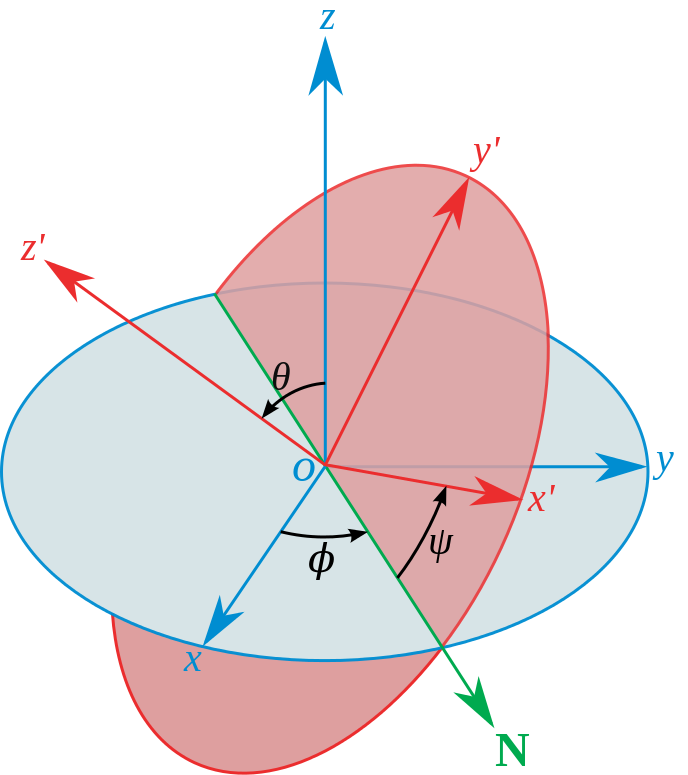
\includegraphics[scale=0.25]{Eulerangles-alternative_filled.png}
\caption{The Euler rotation angles between the rotating
frame $(x', y', 'z')$ and the inertial frame $(x, y, z)$. Image courtesy of
 \citet{WikipediaEuler}.}
\label{fig: Euler}
\end{figure}
This matrix, given values for the Euler angles, transforms from the rotating
frame to the fixed inertial system of coordinates. So for $A^{\textrm{rot}}_b$,
a vector defined in the inertial frame, in the rotating frame the vector has
components given by
\begin{align}
A^{\textrm{in}}_{a} = R^{b}_{\;\;a} A^{\textrm{rot}}_{b}.
\end{align}

\subsection{Evolution of the Euler angles}
\label{sec: evolution of the euler angles}
The Euler angles themselves will evolve with time. To calculate this, we
express the components of the spin-vector $\Omega_a$ along the moving axes ($x', y', z')$. As
shown by \citeauthor{Landau1969}, this results in a set of three ODEs which are
coupled both to the other Euler angles and the components of the spin-vector.
To have solutions both for the motion of the spin-vector in the rotating frame
and the Euler angles we need to solve all six ODEs together. To be specific,
the three Euler rigid-body equations for a biaxial body with a moment
of inertia as defined in Eqn.~\eqref{eqn: MOI} are given by
\begin{align}
\dot{\Omega}_{x} & = \frac{T_x}{I_{0}} -\epsI \Omega_{y} \Omega_{z},
\label{eqn: 6ODE x}
\\
\dot{\Omega}_{y} & = \frac{T_y}{I_{0}} + \epsI \Omega_{x} \Omega_{z},
\label{eqn: 6ODE y}
\\
\dot{\Omega}_{z} & =\frac{T_z}{I_{0}(1+\epsI)}.
\label{eqn: 6ODE z}
\end{align}
The rearranged set of Euler angle ODEs from Equation~(35.1) of
\citet{Landau1969} are given by
\begin{align}
\dot{\phi} & = \frac{\Omega_{x} \sin \psi + \Omega_{y} \cos \psi}{\sin \theta},
\label{eqn: 6ODE phi}
\\
\dot{\theta} & = \Omega_{x} \cos \psi - \Omega_{y} \sin \psi,
\label{eqn: 6ODE theta}
\\
\dot{\psi} & = \Omega_{z} - \dot{\phi} \cos \theta,
\label{eqn: 6ODE psi}
\end{align}
where $\epsI = \Delta I/I_0$ is the deformation of star.
This set of six coupled ODEs can be solved numerically using a time stepper; we
will use the \texttt{rkf45} stepper provided by GSL \citep{gough2009gnu}.
Solutions give the components of the spin-vector in the rotating frame and the
evolution of the Euler angles which can be used to transform rotating frame
quantities into the inertial frame. Unlike the results of Section~\ref{sec:
rotating frame}, numerical solutions to these ODEs require the fast spin frequency
to be resolved and hence require greater computing time.

%The rotation period of the star is several orders of magnitude smaller than the
%precession period, as a result the Euler angles evolve on a much shorter time
%scale than the rotating frame spin components. This is numerically expensive. To
%allow efficient investigations we will therefore consider unrealistic values to
%understand the different types of motion before using realistic values only in
%cases of interest.

\subsection{Initial conditions}
\label{sec: initial conditions}

Solving the rigid-body equations, as in Section~\ref{sec:
rotating frame}, we set
$\Omega_a(t=0)$ to lie in the $x' - z'$ plane at an angle $a_{0}$ to the
$z'$ axis. This gives a set of three initial conditions
\begin{align}
\Omega_{x} & = \omega_{0}\sin(a_{0}), &
\Omega_{y} & = 0, &
\Omega_{z} & = \omega_{0}\cos(a_{0}),
\label{eqn: spin init}
\end{align}
where $\omega_0$ is the initial magnitude of the spin-vector, recalling that
we define $\omega = |\Omega_a|$.

For the Euler angle equations, Eqn.~\eqref{eqn: 6ODE theta} to
Eqn.~\eqref{eqn: 6ODE phi}, the initial conditions need to be chosen carefully
so that the result can be meaningfully interpreted. In particular, we need to
be sure we understand how the inertial frame is orientated. Let us note that
the angular momentum in the two frames are related by
\begin{equation}
\Ji_a = R^{b}_{\;\;a} \Jr_b .
\label{eqn: transform}
\end{equation}
where $R^{b}_{\;\;a}$ is defined in Eqn.~\eqref{eqn: rotation matrix}.

%In the rotating frame, the angular momentum is constant except for small variations
%due to the fact that the torque is not parallel to the angular momentum.
We have already set the initial condition on $\Omega_a$ in Eqn.~\eqref{eqn:
spin init}. Therefore the initial angular momentum in the rotating frame is given by
\begin{equation}
  \Jr_a(t=0) = I^{b}_{\; a} \Omega_b(t=0).
\label{eqn: initial Jr}
\end{equation}
If we set an initial condition on the angular momentum in the inertial frame
$\Ji_a$, then Eqn.~\eqref{eqn: rotation matrix} uniquely defines the initial
Euler angles. We choose to set the initial angular momentum in the inertial
frame to lie along the inertial $z$ axis such that
\begin{equation}
  \Ji_a(t=0) = |\Ji_a| \hat{z}.
\label{eqn: initial Ji}
\end{equation}
The magnitude of the angular momentum is
\begin{equation}
|J_a| = |I^{b}_{\; a} \Omega_{b}|=\omega_{0}I_{0}\sqrt{\sin^{2}a_{0} + \cos^{2}a_{0}(1+\epsI)^2}.
\end{equation}
Using the inverse of Eqn.~\eqref{eqn: transform} and substituting in
Eqn.~\eqref{eqn: initial Jr} and Eqn.~\eqref{eqn: initial Ji} we have
\begin{equation}
\left[ \begin{array}{c}
\sin a_{0} \\
0 \\
(1+\epsI)\cos a_{0}
\end{array}\right] =
\sqrt{\sin^{2} a_{0} + \cos^{2}a_{0}(1+\epsI)^{2}}
\left[ \begin{array}{c}
\sin \psi_{0} \sin \theta_{0} \\
\cos \psi_{0} \sin \theta_{0} \\
\cos \theta_{0}
\end{array}\right].
\label{eqn: 010203}
\end{equation}
This gives us three equations for two unknowns. Our choice to set $\Ji_a$ along
the $z$ axis leaves the initial value of $\phi$ as a free variable.
We set $\phi(t=0) = 0$ without loss of generality.
Rearranging the third component of Eqn.~\eqref{eqn: 010203} yields
\begin{equation}
\theta_{0} = \arccos\left[\frac{(1+\epsI)\cos a_{0}}{ \sqrt{\sin^{2}
        a_{0} + (1+\epsI)^{2}\cos^{2} a_{0}}} \right].
\label{eqn: theta init}
\end{equation}
In the limit $\epsilon_{I} \ll 1$, it can be seen that $\theta_{0} \approx a_{0}$.
For $\psi_0$, we rearrange the first component of Eqn.~\eqref{eqn: 010203} to
give
\begin{equation}
\sin\psi_{0} =\frac{1}{ \sin\theta_{0}}
\frac{\sin a_{0}}{\sqrt{\sin^2 a_{0} + (1+\epsI)^2 \cos^2 a_{0}}}.
\label{eqn: 8283}
\end{equation}
To simplify the first factor, we use the identity $\sin(\arccos(x)) = \sqrt{1 - x^{2}}$
along with Eqn.~\eqref{eqn:  theta init} giving
\begin{equation}
\sin\theta_{0} = \left[\frac{\sin^2 a_{0}}
{\sin^2 a_{0} + (1+\epsI)^2 \cos^2 a_{0}} \right]^{1/2}.
\end{equation}
Inserting this into Eqn.~\eqref{eqn: 8283} and rearranging we find that
\begin{align}
\sin \psi_0 & = \frac{\sin a_{0}}{\left(\sin^{2} a_{0}\right)^{1/2}} \\
 & = \frac{\sin a_{0} }{|\sin a_{0}|} \\
& = \mathrm{sign}(a_{0}),
\end{align}
where by $\mathrm{sign}(x)$ we mean the sign of $x$. Finally, the initial
condition is given by
\begin{align}
\psi_{0} & =\mathrm{sign}(a_{0}) \frac{\pi}{2}.
\label{eqn: psi  init}
\end{align}
We can check the sanity of this result by inserting it into the second component of
Eqn.~\eqref{eqn: 010203} and finding that it balances the left hand side.

In this section, we have defined the appropriate initial conditions for the
system: in addition to Eqn.~\eqref{eqn: spin init} defining the initial spin-vector,
we set the angular momentum in the inertial frame to lie along the
$z$ axis and fix $\phi(t=0)=0$ without loss of generality.  While the
initial conditions on the spin-vector are arbitrary, if the initial Euler angle
are not carefully defined then we do not have a meaningful interpretation for
how the inertial frame is orientated.

\section{Evolving the Euler angles}
\label{sec: evolving the euler angles}

Having defined the coupled ODEs in Eqn.~\eqref{eqn: 6ODE x} to Eqn.~\eqref{eqn:
6ODE psi} and appropriate initial conditions, we can now calculate the evolution
of the spin-vector and Euler angles. The ultimate aim of this section is to go
on to simulate the observable features. However, let us begin by considering the
evolution of the simulation parameters (the components of
$\Omega_a$ and the three Euler angles). We will consider first a torque free
simulation in Section~\ref{sec: biaxial body with no torque} and then add in
the full torque in Section~\ref{sec: biaxial body with torque}.

\subsection{Torque free biaxial body}
\label{sec: biaxial body with no torque}

The set of ODEs given in Eqn.~\eqref{eqn: 6ODE x} to Eqn.~\eqref{eqn: 6ODE psi}
for a biaxial body free of torques have simple analytic solutions
\citep{Landau1969} given by
\begin{align}
    \theta(t) & = \theta_{0} \approx a_{0}, \label{eqn: theta TF}\\
    \phi(t) & = \dot{\phi}t + \phi_{0} = \dot{\phi} t, \label{eqN; phi TF}\\
    \psi(t) & = \dot{\psi}t + \psi_{0}=
 -\frac{\Delta I}{I_0}\dot{\phi} t + \textrm{sign}(a_0)\frac{\pi}{2},
\label{eqn: psi TF}
\end{align}
where in the second equalities we have inserted the initial conditions.
Solution to the rigid-body equations were derived in Eqn.~\eqref{eqn: free
precession x} to Eqn.~\eqref{eqn: free precession z}, transforming these into
the spherical coordinates of the spin-vector we have
\begin{align}
|\Omega_a| & = \omega_0, \label{eqn: omega TF}\\
a & = a_0, \label{eqn: a TF} \\
\varphi & = \epsI\omega_0 \cos(a_0) t,
\label{eqn: varphi TF}
\end{align}
where $\varphi$ is the azimuthal angle of the spin-vector with respect to the
$x'-z'$ plane.  This set of analytic solutions gives us a method to verify our
numerical solver with the appropriate initial conditions.

In Figure~\ref{fig: biaxial body no torque} we present the numerical solutions
for some arbitrary values of the simulation parameters along with the analytic
prediction of Eqn.~\eqref{eqn: theta TF} to Eqn.~\eqref{eqn: varphi TF}. This
demonstrates `almost' perfect agreement between the two: the components of
$\Omega_a$ behave as expected;
%for the Euler angles,
$\phi$ monotonically increases at the spin frequency; $\psi$ decreases at the
slower precession frequency; the polar angle $\theta$ should remain constant
during this simulation, however, we find it varies fractionally by $\sim
10^{-11}$.  This error is caused by the finite numerical precision when
performing the subtraction in Eqn.~\eqref{eqn: 6ODE theta}.
\afterpage{\clearpage}
\begin{figure}[p]
    \centering
\subfloat[Spherical coordinates of the spin-vector in the rotating frame]
         {\includegraphics[width=0.7\textwidth]
         {{Spherical_Plot_Unknown_SpindownTorqueSwitching_1_chi0_8.0000000000e+01_omega0_1.00e+01_epsI3_1.00e-03_AnomTorqueSwitching_1_n_10000_a0_1.5000000000e+01_T_5.00e+03_upsilon_0.00e+00_epsA_0.00e+00_epsI1_0.00e+00_AnomTorque_1}.pdf}} \\
\subfloat[Euler angles ]
         {\includegraphics[width=0.7\textwidth]
         {{Euler_Angles_Unknown_SpindownTorqueSwitching_1_chi0_8.0000000000e+01_omega0_1.00e+01_epsI3_1.00e-03_AnomTorqueSwitching_1_n_10000_a0_1.5000000000e+01_T_5.00e+03_upsilon_0.00e+00_epsA_0.00e+00_epsI1_0.00e+00_AnomTorque_1}.pdf}}
\caption{Solutions to the ODEs defined in Eqn.~\eqref{eqn: 6ODE x} to
Eqn.~\eqref{eqn: 6ODE psi} for a
torque free biaxial star with a deformation of $\epsI = 10^{-3}$. The red
dashed line is the analytic calculation found by \citet{Jones2001}
as given in Eqn.~\eqref{eqn: theta TF} to Eqn.~\eqref{eqn: varphi TF}.}
\label{fig: biaxial body no torque}
\end{figure}

\subsection{Torqued biaxial body}
\label{sec: biaxial body with torque}
To see the difference introducing the EM torque of Eqn.~\eqref{eqn: torque}  makes to the
solutions, in Figure~\ref{fig: biaxial body with torque} we repeat the simulation
plotted in Figure~\ref{fig: biaxial body no torque} with both the anomalous
and spin-down components of the EM torque. The most
striking contrast is the `wobble' in both $\theta$ and $a$; on closer
inspection one also finds this wobble in the other angles, while the magnitude of
$\Omega_a$ both wobbles and undergoes a secular spin-down. To help illustrate
this we have additionally plotted the derivatives $\dot{\phi}$ and $\dot{\psi}$
which were constant in the torque free case. These are calculated numerically,
the numerical errors produce the observed noise.
\afterpage{\clearpage}
\begin{figure}[p]
    \centering
\subfloat[Spherical coordinates of the spin-vector in the rotating frame]
         {\includegraphics[width=0.7\textwidth]
         {{Spherical_Plot_Unknown_SpindownTorqueSwitching_1_chi0_8.0000000000e+01_omega0_1.00e+01_epsI3_1.00e-03_AnomTorqueSwitching_1_n_10000_a0_1.5000000000e+01_T_5.00e+03_upsilon_0.00e+00_epsA_5.00e-04_epsI1_0.00e+00_AnomTorque_1}.pdf}} \\
\subfloat[Euler angles and selected derivatives]
         {\includegraphics[width=0.7\textwidth]
{{Euler_Angles_Unknown_SpindownTorqueSwitching_1_chi0_8.0000000000e+01_omega0_1.00e+01_epsI3_1.00e-03_AnomTorqueSwitching_1_n_10000_a0_1.5000000000e+01_T_5.00e+03_upsilon_0.00e+00_epsA_5.00e-04_epsI1_0.00e+00_AnomTorque_1}.pdf}}
\caption{Solutions to the ODEs defined in Eqn.~\eqref{eqn: 6ODE x} to
Eqn.~\eqref{eqn: 6ODE psi} including the
torque defined in Eqn.~\eqref{eqn: torque} for a biaxial body with
$\epsA=\epsI/2$ and $\epsI=1\times10^{-3}$; the ratio of the precession timescale
to the spin-down age is $\approx 7\times10^{-4}$. Note the x-axis is in units of
$\tauP$, the initial precession period.}
\label{fig: biaxial body with torque}
\end{figure}

These solutions show how, using numerical simulations,
we can easily simulate the effect of the full \citet{Deutsch1955} torque. In the rest
of this chapter, we will discuss how to model the features of a star observed
by pulsar astronomers. This will allow us to change the physics of the star,
i.e.\ by modifying the torque, and directly simulate the effect this has on
the observable properties.


%\paragraph{Convergence test}
%To ensure that the small wobble in $\theta$, which should remain constant, is
%a numerical effect rather than a lack of physics we can plot the fractional
%size of the wobble whilst changing the absolute error tolerance given to the
%ODE stepping procedure. This is done in Figure~\ref{fig: error}
% \begin{figure}[ht]
%\centering
%\includegraphics[scale=0.4]{error_plot.pdf}
%\caption{Fractional size of variations in theta plotted against the relative
%error tolerance given to the stepper.}
%\label{fig: error}
%\end{figure}
%We observe a strange behaviour in which the magnitude of the fractional difference, defined by
%\begin{equation}
%\textrm{Var}(\theta) = \frac{\theta_{\textrm{max}} - \theta_{\textrm{min}}}{|\theta|},
%\end{equation}
%increases exponentially as the error becomes very small. This is due to a
%change in the type of variation of theta, for larger absolute errors we
%observe a period wobble around the expected value of $\theta$. In contrast for
%much smaller absolute errors the solution seems to wander of the mean value
%whilst also undergoing a periodic wobble. We demonstrate this in figure
%\ref{fig: error example} for the two extremes values.
%
%\begin{figure}[ht]
%\centering
%\includegraphics[scale=0.4]{error_example.pdf}
%\caption{Resulsts of simulations with different error tolerances,
%interestingly the smaller absolute error produces greater numerical
%inaccuracy.}
%\label{fig: error example}
%\end{figure}




\section{Precessing pulsars}
\label{sec: precessing pulsars}
Before we move to modelling the physical observable such as phase-residuals,
we need to build our intuition for precession. To do this, we will introduce
the notion of a \emph{reference plane} from which we can decompose the motion of
vectors into rotations about cones.

\subsection{The reference plane}
\label{sec: reference plane}

Considering a biaxial body, let us define $\n^a$ as the \emph{deformation
vector} (a unit vector pointing along the body's symmetry axis), then the
moment of inertia tensor can be written compactly as
\begin{align}
I^{a}_{\;\;b} = I_{0} \delta^{a}_{\;\;b} + \Delta I \n^a \n_b,
\end{align}
where $\delta^{a}_{\;\;b}$ is the Kronecka delta. The principal moments are
given by $I_0=I_{xx}=I_{yy}$ and
$I_{zz} = I_0 + \Delta I$ such that the body is biaxial with $\n_{a}$ lying along
the $\z$ axis. As such, the angular momentum is given by
\begin{align}
J_{a} = I_0 \Omega_a + \Delta I \Omega_z \n_a.
\label{eqn: ang mom}
\end{align}
As found by \citet{Pines1972}, this shows that the three vectors $J_a$,
$\Omega_a$, and $\n_a$ are coplanar in the so-called reference plane as shown in
Figure~\ref{fig: reference plane}.
\begin{figure}[htb]
    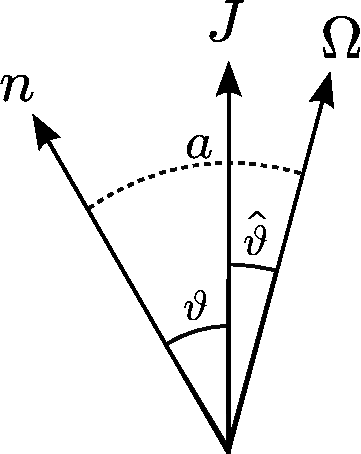
\includegraphics[width=0.25\textwidth]{ReferencePlane.pdf}
    \caption{The reference plane containing the spin-vector $\mathbf{\Omega}$,
    the angular momentum vector $\mathbf{J}$ and the deformation vector $\mathbf{n}$.}
    \label{fig: reference plane}
\end{figure}
In this figure, we have defined the angle between angular momentum and $\n_a$ as
$\theta$, conventionally referred to as the \emph{wobble-angle} of
precession. We have also given $a$, the angle between the $\z$-axis and the
spin-vector as defined in Section~\ref{sec: rotating frame}.

Following \citet{Jones2001}, let us now decompose the angular velocity into the
Euler angle components along the angular momentum and symmetry axis (these
are the same Euler angles as defined in Section~\ref{sec: euler rotation
matrices})
\begin{equation}
  \Omega_a = \dot{\phi}\hat{J}_a + \dot{\psi}\n_{a},
\label{eqn: decomp}
\end{equation}
where $\hat{J}_a$ is a unit vector pointing along the angular momentum. Then,
substituting this into Eqn.~\eqref{eqn: ang mom} we find that
\begin{align}
J_a = I_0 \dot{\phi} \hat{J}_a + \left(I_0 \dot{\psi} + \Delta I \Omega_z\right)\n_a.
\end{align}
Comparing components, we have that
\begin{align}
|J_a| = I_0 \dot{\phi},
\end{align}
and
\begin{align}
\dot{\psi} = -\frac{\Delta I}{I_0} \Omega_z.
\end{align}
To relate the rates of change of the two angles, we can use Eqn.~\eqref{eqn:
6ODE psi}, giving
\begin{align}
\dot{\psi} = - \frac{\Delta I}{I_0 + \Delta I} \dot{\phi} \cos\theta
\approx -\frac{\Delta I}{I_0} \dot{\phi} = -\epsI \dot{\phi}
\label{eqn: psi phi}
\end{align}
where we have approximated assuming $\Delta I \ll I_0$ and $\theta \ll 1$ in
the last step.

We can relate both of these frequencies to the angular frequency $\omega = |\Omega_a|$.
First, from the cosine rule we have that
\begin{align}
|\Omega_a|^{2} = \dot{\phi}^{2}+\dot{\psi}^{2} - 2\dot{\phi}\dot{\psi}\cos\theta.
\end{align}
and so rearranging and neglecting terms of order $\epsI^{2}$, we have that
\begin{align}
\dot{\phi} \approx \frac{\omega}{\sqrt{1- 2\epsI\cos\theta}}.
\label{eqn: phi dot}
\end{align}
Since $\epsI \ll 1$, we know that $\dot{\phi}$ is approximately the fast spin frequency
of the star $\omega$. Then from Eqn.~\eqref{eqn: psi phi}, we see that $\dot{\psi} \ll \omega$
is a much slower frequency, the precession frequency.

%From the previous section we learnt that any vector fixed in the rotating frame
%can be transformed into the inertial frame by the Euler angle rotation matrix,
%Eqn.~\eqref{eqn: rotation matrix}. For torque free precession $\theta$ is a
%constant \citep{Landau1969}; therefore when viewed in the inertial frame, any
%fixed vector in the rotating frame can be understood as undergoing two motions:
%keeping $\phi$ fixed and increasing $\psi$ rotates the vector in a cone
%about the $\n_{a}$ axis at frequency $\dot{\psi}$; holding
%instead $\psi$ fixed and increasing $\phi$ sweeps the vector about a cone
%centred around the $\hat{J}_a$ axis at frequency
%$\dot{\phi}$. The motion of the fixed vector is the superposition of these two
%rotations; the $\psi$ rotation is referred to as precession and happens at a
%slower frequency as seen from Eqn.~\eqref{eqn: psi phi}.

We will now discuss the effect of free precession on the motion of $\m_a$, the
magnetic dipole. We will do this initially by studying the evolution of the
dipole in the inertial frame via the Euler angle rotations and then we will
return to this reference frame picture in Section~\ref{sec: understanding the
motion of m} to provide a deeper intuitive understanding.

\subsection{Dynamics of the magnetic dipole}

Numerical solutions to Eqn.~\eqref{eqn: 6ODE x} to Eqn.~\eqref{eqn: 6ODE psi}
allow us to calculate the motion of any quantity in the inertial frame from
which the neutron star is observed.  This can be used, for example, to
calculate the motion of the spin-vector as seen by an observer for any
arbitrary torque. However, pulsar astronomers observe the pulsar through the
pulsations of EM emission. If this emission is collinear with the dipole, then
it points along the unit vector of the magnetic dipole $\m_a$. Therefore, we
are particular interested in the motion of $\m_a$ in the inertial frame. This
system was first studied in the follow way by \citet{bisnovatyi1990model}, but
here we follow the treatment by \citet{Jones2001}.

In the rotating frame, we set $\m_a$ to lie at an angle $\chi$ to the $z'$ axis
with unit vector $[\sin(\chi), 0, \cos(\chi)]$ without loss of generality.
Using Eqn.~\eqref{eqn: rotation matrix}, the Euler
rotation matrix, we can transform to the inertial frame; the components of the
magnetic dipole in the inertial frame are
\begin{equation}
\m_a =
\left[\begin{array}{c}
\cos\phi\cos\psi\sin\chi - \sin\phi \cos \theta \sin \psi \sin \chi
+ \sin \phi \sin \theta \cos \chi \\
\sin\phi\cos\psi\sin\chi + \cos\phi \cos \theta \sin \psi \sin \chi
- \cos \phi \sin \theta \cos \chi \\
\sin\theta \sin\psi \sin\chi + \cos\theta \cos \chi
\end{array}\right].
\label{eqn: m inertial}
\end{equation}
We define two angles $\Phi$ and $\Theta$
which describe the polar and azimuthal angles of $\m_a$ in the inertial frame.
From Eqn.~\eqref{eqn: m inertial} the azimuthal angle is given by
\begin{equation}
    \Phi = \arctan\left(\frac{\m_{y}}{\m_{x}}\right) =
    \phi - \frac{\pi}{2} + \arctan\left[\frac{1}{\cos\theta}
    \left(\frac{\cos\psi \tan \chi}{\tan\theta -
            \sin \psi \tan\chi }\right)\right],
\label{eqn: Phi}
\end{equation}
while the polar angle is
\begin{equation}
\Theta = \arccos(\m_{z}) = \arccos(\sin \theta \sin \psi \sin \chi + \cos \theta \cos \chi ).
\label{eqn: Theta 2}
\end{equation}

Eqn.~\eqref{eqn: Phi} and Eqn.~\eqref{eqn: Theta 2} are exact results and
we will use them later in this chapter to model the observable features such
as the phase residuals and spin-down rate.
Specifically, given a numerical solution to our system of coupled ODEs, i.e.\ the evolution of the spin-vector and three Euler angles, we can use these two
equations to describe the evolution of the magnetic dipole orientation in the
inertial frame. Before we do this, let us now build some feeling for the dynamics of
the magnetic dipole in the inertial frame in the torque free case.

Using our numerical solution, we simulate a star without any EM torque. The
resulting solutions for the Euler angles can then be substituted into Eqn.~\eqref{eqn: Theta 2}
to give the evolution of $\Theta$. This is done for three choices of $\theta$
and $\chi$ in Figure~\ref{fig: polar angle variations}.
\begin{figure}[htb]
\centering
  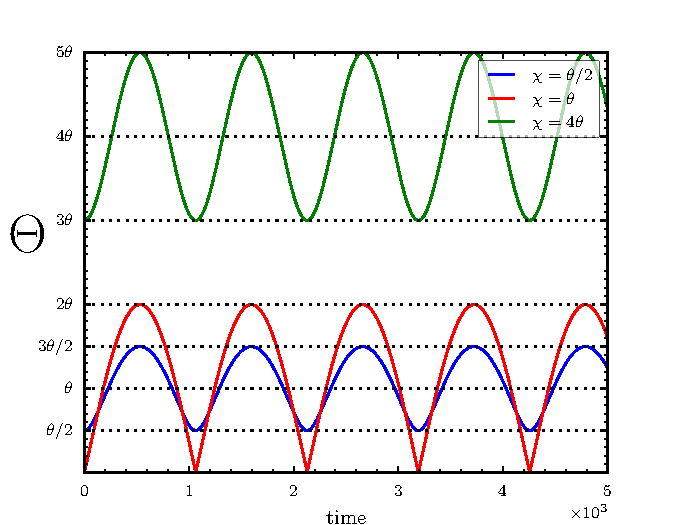
\includegraphics[width=0.9\textwidth]{polar_angle_variation_with_chi.pdf}
\caption{The effect of free precession on the polar angle of the dipole $\m_a$
as given by Eqn.~\eqref{eqn: Theta 2} for three choices of $\chi$ and
$\theta$.}
\label{fig: polar angle variations}
\end{figure}
From this figure, we see that the polar angle is modulated at the precession
period, $\tauP$. In the next section, we will provide a deeper understanding
of the size of modulations and the significance in the choice
of $\theta$ and $\chi$.

The observed spin frequency of a pulsar is the rate with which observers measure the
observed pulsations. Usually we think of this as exactly equivalent to the
rotation frequency $\omega/2\pi$. However, for a precessing star the observed
frequency is not given by $\omega/2\pi$ due to the additional motions of precession.
Instead, the observer would fit a timing model to the TOAs as the
pulse passes through the plane containing the observer and the angular momentum vector,
the phase of which is $\Phi$. So the frequency measured would be given by the
first derivative of $\Phi$:
\begin{equation}
\dot{\Phi} = \dot{\phi}
+ \frac{\sin\chi \left(
\dot{\psi} (\cos\theta\sin\chi - \sin \psi \sin \theta \cos\chi) +
\dot{\theta} \cos\psi (\cos\theta\cos\chi - \sin \psi \sin \theta \sin\chi)\right)
}{(\sin\theta \cos \chi - \cos \theta \sin \psi \sin \chi)^{2} + \cos^{2}\psi \sin^{2} \chi}.
\label{eqn: Phi_dot}
\end{equation}
This is the \emph{instantaneous electromagnetic frequency}; an observer
will measure the time averaged value of $\dot{\Phi}$ as the `spin frequency' of
the star.

In Figure~\ref{fig: frequency variations} we plot the frequency modulations for
the three choices of $\theta$ and $\chi$ used in Figure~\ref{fig: polar angle variations}.
Again, we see modulation at the precession period; in the following section, we
will provide a deeper understanding of these modulations and our choices of
$\theta$~and~$\chi$.
\begin{figure}[htb]
\centering
  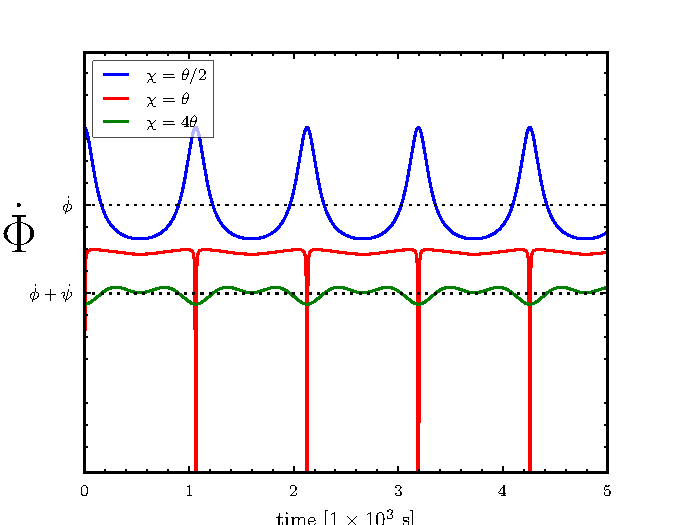
\includegraphics[width=0.9\textwidth]{frequency_variation_with_chi.pdf}
\caption{The effect of free precession on the instantaneous electromagnetic
frequency given by Eqn.~\eqref{eqn: Phi_dot} for three choices of $\chi$ and
$\theta$.}
\label{fig: frequency variations}
\end{figure}


\subsection{Understanding the dynamics of the magnetic dipole}
\label{sec: understanding the motion of m}

We will now return to the reference plane picture discussed in Section~\ref{sec:
reference plane}. In particular, we provide a detailed description of
the motion of $\m_a$ as seen by the observer and use this to explain the
modulations seen in Figure~\ref{fig: polar angle variations} and Figure~\ref{fig:
frequency variations}.

Firstly, let us state our assumption that EM radiation is emitted along the
dipole axis $\m_a$ such that it is this axis from which an observer sees
pulsations.  From the decomposition of the spin-vector in Eqn.~\eqref{eqn:
decomp}, the motion of the magnetic dipole, a vector fixed in the rotating
frame, when viewed in the inertial frame, can be understood as the
superposition of two rotations.  If we hold $\phi$ fixed, then $\m_a$ rotates
in a cone of half-angle $\chi$ about the symmetry axis $\n_a$ at the slow
precession angular frequency $\dot{\psi}\approx -\epsI \omega$ and we call this
the \emph{precession cone}. On the other
hand, if we hold $\psi$ fixed, then $\n_a$ rotates in a cone of half-angle
$\theta$ about $J_{a}$ at the angular frequency $\dot{\phi} \approx \omega$.
Still holding $\psi$ fixed, since $\m_a$ is necessarily always at a fixed angle
$\chi$ to $\n_a$, it too will be swung in a cone of half-angle $\Theta$ (as
given in Eqn.~\eqref{eqn: Theta 2}) about the angular momentum vector with
angular frequency $\dot{\phi}$; let us define this to be the \emph{dipole
cone}. Now, $\psi$ evolves at a slower rate to $\phi$ by a factor $\epsI$,
moreover, the negative relation between them in Eqn.~\eqref{eqn: psi phi},
indicates that the precession cone counter-rotates with respect to the
dipole cone. If we consider the effect of both rotations together and their effect on the 
dipole cone, we see that the
half-angle of the dipole cone $\Theta$ is modulated by precession (see
Figure~\ref{fig: polar angle variations}): as $\m_a$ rotates about the dipole
cone, the cone gradually opens and closes at the precession period. The rate at
which $\m_a$ rotates about the dipole cone is given by $\dot{\Phi}$, as given
by Eqn.~\eqref{eqn: Phi_dot}. Similarly this is also modulated by precession as
shown in Figure~\ref{fig: frequency variations}. 

The resulting motion of the dipole cone is best understood by considering three
choices of $\chi$ and $\theta$: $\chi < \theta$, the special case $\chi =
\theta$, and $\chi > \theta$. We illustrate the projection of the precession cone swept
out by $\m_a$ about $\n_a$ (in red) and the cone swept out by $\n_a$ about $J_a$ onto
the reference plane for the three orderings of $\chi$ and $\theta$ in
Figure~\ref{fig: cones}. Note that the dipole cone is not shown here.
\begin{figure}[ht]
\centering
	\subfloat[$\chi < \theta$]{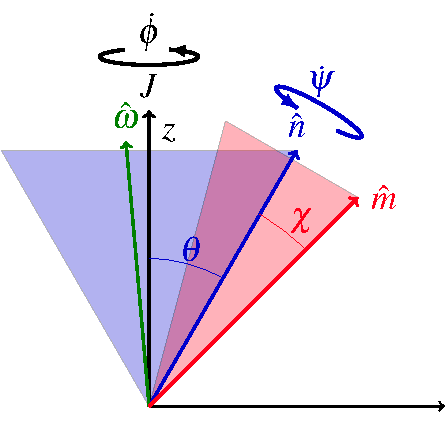
\includegraphics[width=0.33\textwidth]
    {chi_less_theta.pdf}}
	\subfloat[$\chi = \theta$]{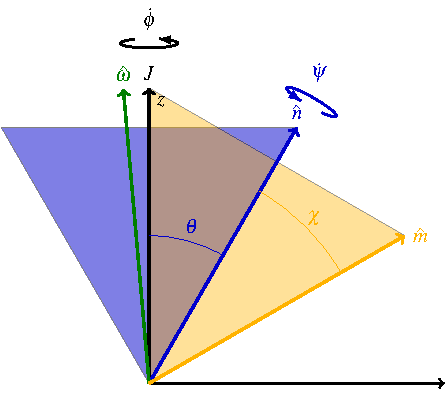
\includegraphics[width=0.33\textwidth]
    {chi_equal_theta.pdf}}
	\subfloat[$\chi > \theta$]{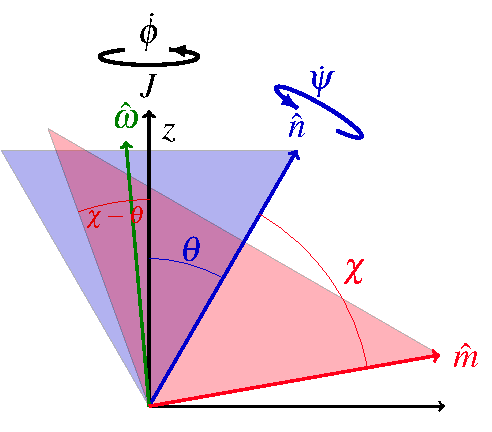
\includegraphics[width=0.33\textwidth]
    {chi_more_theta.pdf}}
\caption{Diagrams depicting the projections of the cone swept out by $\m_a$
about $\n_a$ (in red) and the cone swept out by $\n_a$ about $J_a$ (in blue)
onto the reference plane for torque free precession. We show the three
orderings of $\chi$~and~$\theta$.}
\label{fig: cones}
\end{figure}

Let us now describe
the evolution of the dipole cone for the three cases in Figure~\ref{fig: cones}.
We will discuss in particular the choices of $\chi$ and $\theta$ which were used
in Figure~\ref{fig: polar angle variations} and Figure~\ref{fig: frequency variations}
for the variations in polar angle and instantaneous electromagnetic frequency
respectively.
\begin{itemize}
\item The $\chi < \theta$ case ($\chi = \theta/2$): the precession cone is
narrow and does not extend over the angular momentum vector. The polar angle
$\Theta$ of the dipole cone oscillates periodically between $\theta+\chi$ and
$\theta-\chi$ during a precession cycle, as shown in Figure~\ref{fig: polar angle
variations}.  The spin frequency $\dot{\Phi}$, as shown in Figure~\ref{fig: frequency
variations}, has an average value of $\dot{\phi}$ and oscillates about this
value. Comparing with the $\Theta$ variations demonstrates these oscillations
are locked in phase with the rotation of $\m_a$ in the precession cone. Recalling
that the precession cone counter-rotates with respect to the spin cone, at
$\theta+\chi$ the precession cone motion acts in the opposing direction to the
spin cone. This causes a reduction in the spin frequency away from the average.
By contrast, at $\theta-\chi$ the precession cone motion acts in the same
direction as the spin cone producing an increase in the spin frequency above
the average.

\item The $\chi = \theta$ case: in this special case the angular momentum vector sits exactly
on the side of the precession cone. This suggests that at certain precessional phases $\m_a$ can align exactly with
the angular momentum. When this happens the spin frequency tends to zero manifesting as sharp dips in the
spin frequency; at the same time the polar angle tends to zero.

\item The $\chi > \theta$ case ($\chi = 4\theta$): The precession cone now extends over the
angular momentum vector. This means it always acts to reduce the spin
frequency; as a result the spin frequency has an average value of
$\dot{\phi} + \dot{\psi}$. The polar angle can vary between $\theta+\chi$ and
$\chi-\theta$. For $\chi$ close to $\theta$ the deviations away from the
average are large while as $\chi$ increases the deviations get smaller as
the half angle of the dipole cone increases.
\end{itemize}

\subsection{The effective wobble angle}
\label{sec: wobble angle}
The angle $\theta$ (see Figure~\ref{fig: reference plane}) is referred to as the
\emph{wobble angle} since, in torque-free precession, its magnitude determines
the `amount' of precession. Taking Eqn.~\eqref{eqn: ang mom} at an instant when
$\Omega_y=0$ without loss of generality it can be shown that
\begin{align}
\tan\theta  = \frac{I_0}{I_0 + \Delta I} \tan(a) = \frac{1}{1+\epsI}\tan(\theta + \hat\theta).
\end{align}
Using the angle sum identity for $\tan(\theta + \hat{\theta})$ and expanding
about $\epsI=0$ it can be shown \citep{Jones2001} that
\begin{align}
\hat{\theta} \approx \epsI\sin\theta\cos\theta.
\label{eqn: theta hat theta}
\end{align}
Then for $\theta \ll 1$, we have that $a\approx \theta + \mathcal{O}(\epsI)$.

When including the EM torque the wobble angle
does not have the intuitive interpretation of the `amount' of precession.  In
particular, the anomalous part of the torque defined in Eqn.~\eqref{eqn: torque}
can be understood to create an effective rotating frame as shown in Section~\ref{sec:
effective body frame}. This means that solutions exist which appear to undergo
`persistent precession' where $\theta \approx a\ne0$ such that the body remains
misaligned from the principal axes of its moment of inertia tensor. However, we
demonstrated that in fact the body has aligned with the principal axes of
it \emph{effective} moment of inertia tensor.

Let us then define an effective wobble angle
\begin{align}
\wobbleangle = \theta - \beta,
\label{eqn: effective wobble angle}
\end{align}
which describes the amount of precession under the full electromagnetic torque.
That is, we rotate the usual wobble angle by $\beta$ defined in
Eqn.~\eqref{eqn: beta}. In the limit where $\beta \rightarrow 0$ we recover the
usual wobble angle referred to by \citet{Jones2001} $\theta = \wobbleangle$.
But, if the effects of the anomalous torque are important (see Chapter~\ref{sec:
rotating frame} for examples of when this is the case), then the effective wobble
angle $\wobbleangle$ will measure the amount of precession (i.e.\ its magnitude
determines the amplitude of precession). This definition will be used later on
when setting up solutions which initially have a minimal amount of precession.



%\subsection{Pulse frequency and polar angle under torqued precession}
%Having a physical understanding of why $\Theta$ and $\dot{\Phi}$ evolve under
%free precession as in Figure~\ref{fig: polar angle variations} and Figure~\ref{fig:
%frequency variations}, we will study what happens to such a system when
%including the effects of the EM torque.
%
%In Figure~\ref{fig: polar angle variations with torque}  we give the variations in
%the polar angle under torqued precession.The torque introduces two
%additional effects: $\dot{\Phi}$ the instantaneous electromagnetic frequency
%decays slowly, this is caused by the spin-down torque and is full agreement
%with what we expect; a fast sinusoidal oscillation in $\dot{\Phi}$ on the spin
%timescale, observable as a broadening of the line, is a result of the
%anomalous torque. As for the polar angle $\Theta$ the anomalous torque causes
%slight changes in the limits of the sinusoidal variation. Both the anomalous
%torque effects can be understood by realising that this effectively adds a
%triaxiality into the moment of inertia tensor. % needs more explanation
%
%\begin{figure}[ht]
%\centering
%	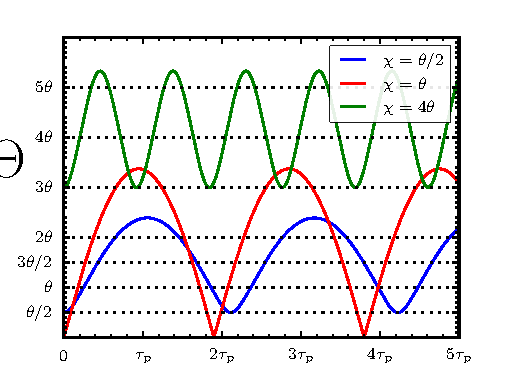
\includegraphics[width=0.7\textwidth]{polar_angle_variation_with_chi_inc_torque.pdf}
%\caption{Variations in the polar angle of the dipole $\m_a$ under torqued precession}
%\label{fig: polar angle variations with torque}
%\end{figure}
%
%\begin{figure}[ht]
%\centering
%	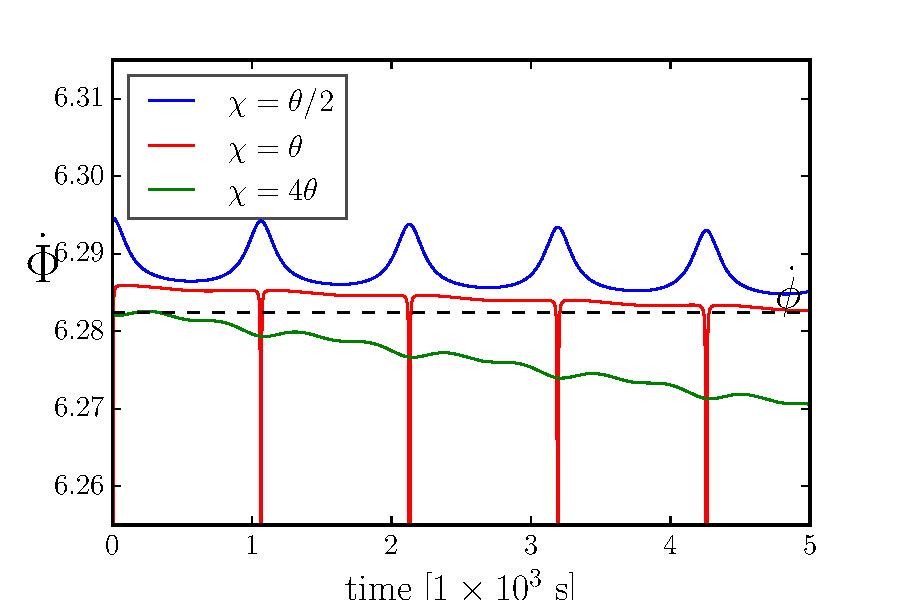
\includegraphics[width=0.7\textwidth]{frequency_variation_with_chi_inc_torque.pdf} \\
%\caption{Variations in the spin-frequency of the dipole $\m_a$ under torqued precession}
%\label{fig: frequency variations with torque}
%\end{figure}

\section{Observable features: the phase residual}
\label{sec: observable features: timing residuals}

The principal observational quantity reported on for a pulsar is the timing
residual. This is the difference between the measured TOA of a pulse and a
timing model of the pulsar as discussed in Section~\ref{sec: pulsar timing
methods}.  The phase modulation of pulsars due to precession was first modelled
in response to periodic variations observed in the frequency of the Crab pulsar
\citep{Ruderman1970, chiuderi1970shape}. Precession as a candidate for periodic
variations in Hercules X-1 was studied by \citet{bisnovatyi1990model} and
\citet{bisnovatyi1993period}. Since then, there has been extensive work in the
literature: \citet{Nelson1990} calculated phase residuals both analytically and
numerically for freely precessing stars; torqued precession was considered for
a general torque by \citet{Jones1988excitation} and \citet{Cordes1993} and then
for the \citet{Deutsch1955} torque by \citet{Melatos1999, Melatos2000}.  In
this section, we will calculate residuals by calculating the pulsar phase from
our numerical model and then fitting and removing a Taylor expansion. This
means that we capture the data collection methods present in any real data.
Note that timing residuals and phase residuals are equivalent up to factors of the
pulse period. We will discuss this once we have defined the phase
residual.

The azimuthal angle $\Phi$ given in Eqn.~\eqref{eqn: Phi} gives us the phase of
the magnetic dipole. For the observer, the pulsation occurs when the dipole
passes through the plane containing the observer and the angular momentum
vector.  We can always reorient the observer such that the pulsation occurs
every time $\Phi$ is a multiple of $2\pi$. In this way, $\Phi$ is also the
phase of the observed pulsations. To generate $\Phi$ we define the star's
properties i.e.\ the magnetic field and initial angles, then numerically evolve
Eqn.~\eqref{eqn: 6ODE x} to Eqn.~\eqref{eqn: 6ODE psi}. The resulting time
series of the spin-vector components and Euler angles are then substituted into
Eqn.~\eqref{eqn: Phi} to generate the exact phase.

Following the methods used by observers, we define our `timing model' as
a Taylor expansion of the phase about some reference time $\tref$ up to $\ddot{f}$:
\begin{equation}
    \Phifit(t; \tref, \f, \fdot, \fddot) =
    2\pi \left(\f(t - \tref) +
                          \frac{\fdot}{2!}(t-\tref)^{2} +
                          \frac{\fddot}{3!}(t-\tref)^{3}
                          \right),
\label{eqn: TR taylor expansion}
\end{equation}
with the timing properties ($f$, $\dot{f}$, $\ddot{f}$) as free parameters.
Higher order terms can be included, as discussed in Section~\ref{sec: timing noise
observations}, but here we truncate at $\ddot{f}$. We do not include an initial
phase since we can arbitrarily define our reference time to coincide with a
pulsation such that the initial phase is zero.  Unlike pulsar astronomers, we
do not need to worry about other corrections such as the motion of the Earth
since $\Phi$ is given in the inertial frame.

The phase residual is then the difference between the exact phase
and the fitted phase
\begin{equation}
  \Delta\Phi(t) = \Phi(t) - \Phifit(t; \tref, \f, \fdot, \fddot).
\end{equation}
We then use a least-squares fitting method to minimise the root mean squared
error of the phase residual. The fitted coefficients $\{\f, \fdot,
\fddot\}$ constitute our best-fit phase model: the best fit to the data
$\Phi(t)$ of a power law spin-down model.  It is worth noting that a residual
depends on which section of data was used in the fit.

In this work, we will report only on phase residuals. However, we note that the
phase residual can also be re-scaled to give the timing residual by calculating
the residual as a fraction of a cycle then multiplying by the period:
\begin{equation}
    \Delta T = \frac{\Delta\Phi(t)}{2\pi} P.
    \label{eqn: phase to timing}
\end{equation}

In the following subsections, we will compare analytic results for the phase
residuals due to precession with our numerical results found by fitting and
removing a polynomial. As shown in Section~\ref{sec: understanding the motion of m}
the form of solution will depend on whether $\chi < \theta$ or $\chi > \theta$.
Of these two choices, \citet{Jones2001} concluded that `the wobble angle of
rapidly rotating stars are limited to small values for the finite crustal
breaking strain'; following this reasoning we will limit our study to the
$\chi > \theta$ case although the numerical code is capable of finding solutions
for either.

\subsection{Effect of precession on the phase residual}

The effect of free precession on phase residuals was first considered by
\citet{Nelson1990}; since the modulations are due to the geometric effect of
precession, they are referred to as the \emph{geometric effect}. To calculate a
phase residual, \citet{Jones2001} subtracted the secular phase evolution from
Eqn.~\eqref{eqn: Theta 2} and, found that the phase residual when $\chi > \theta$
is given by
\begin{equation}
    \Delta\Phi_{49}(t) = -\theta \cot\chi\cos\left(\dot{\psi}t + \frac{\pi}{2}\right),
    \label{eqn: Jones 49}
\end{equation}
where the subscript here refers to the equation number of \citet{Jones2001}.
For a precessing star $\dot{\psi}$ is given by Eqn.~\eqref{eqn: psi phi} and
the initial value of the cosine argument is $\psi(t=0)=\pi/2$ as derived in
Section~\ref{sec: initial conditions}.

Equation \eqref{eqn: Jones 49} is calculated in the absence of any EM torque.
Nevertheless, it is still appropriate when a torque is applied provided
that the geometric effect is stronger that any other (this is discussed in
the next few sections). As such, we begin by simulating a star with the
properties listed in Table~\ref{tab: PR 49}.
The resulting phase residual, in cycles, is given in Figure~\ref{fig: PR 49}.
This figure shows strong agreement between the numerical result and the
analytic prediction of Eqn.~\eqref{eqn: Jones 49}.

\begin{table}[htb]
\centering
\begin{tabular}{ccl}
\multicolumn{3}{c}{Simulation parameters} \\
\hline
$\omega_0$  &=& 10.0 rad/s\\
$B_0$  &=& ${1.0}{\times} 10^{13}$ G \\
$\chi$  &=& 50.00$^{\circ}$ \\
$a_0$ &=& 2.00$^{\circ}$ \\
$\tilde{\theta}$ &= & 2.00$^{\circ}$ \\
$\mathcal{A}_{\mathrm{EM}}$ &= & ${4.3}{\times} 10^{-6}$
\end{tabular}
\caption{Simulation parameters used for the phase residual plotted in
Figure~\ref{fig: PR 49}. Note that $\Aem$ is the electromagnetic amplification
factor defined later in Eqn.~\eqref{eqn: EM amplification}.}
\label{tab: PR 49}
\end{table}

\begin{figure}[htb]
\centering
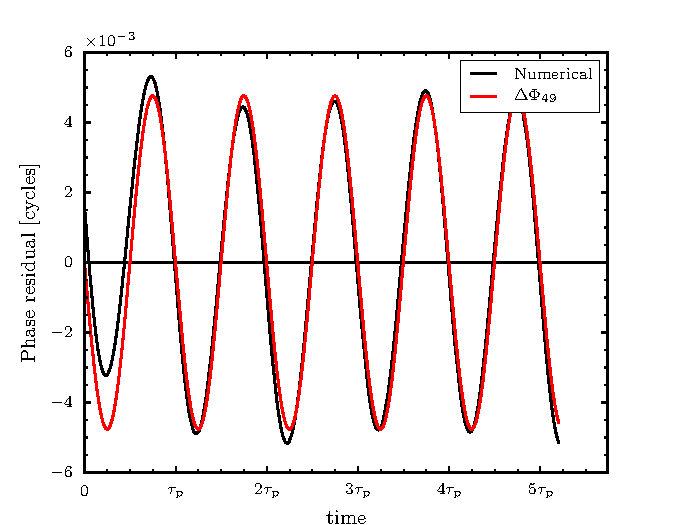
\includegraphics[width=0.8\textwidth]{49_verification}
\caption{The simulated phase residual in cycles for a simulated star with the
properties described in Table~\ref{tab: PR 49}. We also plot the corresponding
analytic prediction of Eqn.~\eqref{eqn: Jones 49} which is the geometric effect
of precession on the phase residual.}
\label{fig: PR 49}
\end{figure}

\subsection{Effect of torqued precession on the phase residual: electromagnetic amplification}
\label{sec: phase residual torqued}

The geometric effects of precession can be amplified by the EM torque \citep{Cordes1993}.
Using a simple description based on a vacuum point-dipole spin-down torque,
and calculating the departure from a non-precessing power-law spin-down,
the amplified phase residuals are given by
\begin{align}
\Delta\Phi_{63} = -\frac{1}{\pi}\left(\frac{\tau_{P}}{P}\right)
                               \left(\frac{\tau_{P}}{\tauAge}\right)
                               \theta
                               \cot\chi
                               \sin(\dot{\psi} t + \pi/2),
\label{eqn: Jones 63}
\end{align}
where $\tauAge=|\dot{\Phi}/\ddot{\Phi}|$, note this is equivalent up to a factor
2 with the original definition in Eqn.~\eqref{eqn: tauAge definition}; here,
we will use the definition from \citet{Jones2001} for consistency.
This result is derived in \citet{Jones2001} for the magnitude of modulations.
Here we keep the exact time evolution behaviour intact. We will derive this
expression later on in Section~\ref{sec: derivation of the spin-down rate}.
Notably, we can write the magnitude of modulations in term of Eqn.~\eqref{eqn:
Jones 49} as
\begin{equation}
    |\Delta\Phi_{63}| = \frac{1}{\pi}\left(\frac{\tau_{P}}{P}\right)
    \left(\frac{\tau_{P}}{\tauAge}\right)
                                    |\Delta\Phi_{49}|
\label{eqn: Jones 63 mag}
\end{equation}
The two ratios of timescales define an `amplification factor'
\begin{equation}
    \mathcal{A}_{\mathrm{EM}} = \left(\frac{\tau_{P}}{P}\right)
                                \left(\frac{\tau_{P}}{\tauAge}\right).
\label{eqn: EM amplification}
\end{equation}
The amplification, as first noted by \citet{Cordes1993}, increases the
magnitude of phase residuals for young pulsars with short periods. It is worth
noting however, that there is a relative phase difference between
Eqn.~\eqref{eqn: Jones 49} and Eqn.~\eqref{eqn: Jones 63}.

To verify this amplification, we simulate a star using the properties in
Table~\ref{tab: PR 63} for which the amplification factor is greater than
unity.
The resulting phase residual is plotted in Figure~\ref{fig: PR 63} along with the
predictions of Eqn.~\eqref{eqn: Jones 63} and Eqn.~\eqref{eqn: Jones 49}. This
clearly demonstrates that the amplified residuals agree with the results
calculated numerically while the geometric effect is both out of phase and
has a smaller amplitude by a factor $\Aem/\pi$, where the amplification factor is
given in Table~\ref{tab: PR 63}.

\begin{table}[htb]
\centering
\begin{tabular}{ccl}
\multicolumn{3}{c}{Simulation parameters} \\
\hline
$\omega_0$  &=& $10^{4}$ rad/s\\
$B_0$  &=& $ 10^{14}$ G \\
$\chi$  &=& 50$^{\circ}$ \\
$a_0$ &=& 2$^{\circ}$ \\
$\mathcal{A}_{\mathrm{EM}}$ &= & $43$
\end{tabular}

\caption{Simulation parameters used for the phase residual plotted in
Figure~\ref{fig: PR 63}.}
\label{tab: PR 63}
\end{table}

\begin{figure}[htb]
\centering
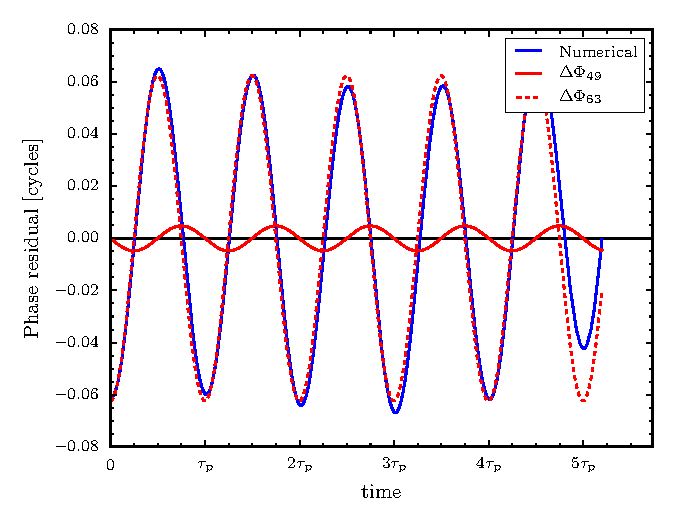
\includegraphics[width=0.8\textwidth]{63_verification}
\caption{The simulated phase residual in cycles for a simulated star with the
properties described in Table~\ref{tab: PR 63}. We also plot the corresponding
analytic prediction for the geometric effect of precession given by
 Eqn.~\eqref{eqn: Jones 49} and the EM amplification of precession given by
Eqn.~\eqref{eqn: Jones 63} which is the appropriate prediction for this simulation.}
\label{fig: PR 63}
\end{figure}

\section{Observable features: the spin-down rate}
\label{sec: observable features: spin-down rate}

The derivatives of the phase (the frequency, spin-down rate, etc.) display
similar periodic departures from their secular evolutions; in the same way as
for the phase residual, these periodic modulations can be amplified by the
EM torque. In Figure~\ref{fig: frequency variations} we have already shown
the modulations of the frequency due to free precession. However,
long term modulations of the frequency (on top of the usual secular spin-down),
are not reported in the literature and so we will not consider them further.
The second physical observable that we will consider is the spin-down rate
for which modulations are reported in the literature.

PSR~B1828-11 is a normal radio pulsar which displays strong periodic modulation
in its spin-down rate. This has been modelled analytically by several authors
\citep{Stairs2000, Jones2001, Link2001, Akgun2006} who all found that the timing
residuals and spin-down rate modulations were consistent with EM-dominated
precession. We can confirm this by noting that the inferred precession period for this
pulsar is $\tauP \approx 500$~days, the period is $P\approx0.405$~s, and
the spin-down age is $\tauAge \approx P/\dot{P} \approx 2.1 \times10^{5}$~yrs (values
taken from the ATNF catalogue \citet{ATNF}), therefore the EM amplification factor
defined in Eqn.~\eqref{eqn: EM amplification} is
\begin{align}
\Aem \approx 700.
\end{align}

In this section, we will derive an analytic model for the spin-down rate of a
precessing pulsar dominated by the EM torque; this model will be used in
Chapter~\ref{sec: testing models} to test the precession model for
PSR~B1828-11. Then, we will compare this analytic model with a spin-down rate
calculated numerically. We will not consider the geometrically dominated
spin-down rate modulations. Further details on that subject can be found in
\citet{Jones2001}.

\subsection{Derivation of the precession spin-down rate}
\label{sec: derivation of the spin-down rate}
Let us now derive the spin-down rate for a precessing pulsar under a vacuum
point-dipole spin-down torque. Equivalent derivations can be found in
\citet{Link2001} and \citet{Jones2001}; in this derivation we will start
with a generalisation of vacuum point-dipole torque to allow for a braking
index $n\ne3$, but retain the angular dependence. The following provides
the complete details of a calculation we will use later in Chapter~\ref{sec:
testing models} and which was published in \citet{Ashton2016}.

Our generalisation of the vacuum point-dipole spin-down torque can be written as
\begin{align}
\ddot{\Phi} = -k \dot{\Phi}^{n} \sin^{2}\Theta,
\label{eqn: EM DE}
\end{align}
where $k$ is a positive constant. From Eqn.~\eqref{eqn: Theta 2} we have that
\begin{align}
\cos\Theta = \sin\theta \sin \psi(t) \sin \chi + \cos\theta \cos\chi.
\end{align}
Rearranging and expanding about $\theta = 0$ and keeping terms up to
$\mathcal{O}(\theta^{2})$, we find
\begin{align}
\sin^{2}\Theta & =
\left[
\sin^{2}\chi + \theta^{2}\left(\cos^{2}\chi - \frac{\sin^{2}\chi}{2}\right)
\right]
- 2\theta \sin\chi\cos\chi \sin\psi(t)
 + \frac{1}{2}\theta^{2}\sin^{2}\chi\cos(2\psi(t)),
\label{eqn: sin 2 Theta}
\end{align}
where the first term, in square brackets, is a constant while the second two
terms provide the first and second harmonic modulations in $\sin^{2}\Theta$.

In order to find approximate solutions to Eqn.~\eqref{eqn: EM DE}, we begin by
defining the time-averaged (constant) value of $\sin^{2}\Theta$ as
\begin{align}
\sin^{2}\Theta_0 =
\sin^{2}\chi + \theta^{2}\left(\cos^{2}\chi - \frac{\sin^{2}\chi}{2}\right),
\label{eqn: sin2Theta0}
\end{align}
then solving Eqn.~\eqref{eqn: EM DE} with this constant value we get
\begin{align}
\dot{\Phi}(t) = \left[\frac{1}{\dot{\Phi}_0^{(n-1)}}
+ (n-1)k\sin^{2}\Theta_0 t \right]^{\frac{-1}{n-1}},
\label{eqn: zeroth order soln}
\end{align}
where $\dot{\Phi}_0 = \dot{\Phi}(0)$. Now the spin-down timescale is
\begin{align}
\tauAge = \frac{|\dot{\Phi}_0|}{|\ddot{\Phi}_0|}
\approx \frac{1}{k|\dot{\Phi}_0|^{(n-1)} \sin^{2}\Theta_0},
\end{align}
again we note that this differs by a factor of 2 to the definition in
Eqn.~\eqref{eqn: tauAge definition}, we use this definition here for
consistency with \citet{Jones2001}. Rearranging gives
\begin{align}
k = \frac{1}{\tauAge \dot{|\Phi}_0|^{(n-1)} \sin^{2}\Theta_0}.
\end{align}
Then Eqn.~\eqref{eqn: zeroth order soln}, our zeroth-order solution to the
spin-down (under a constant $\Theta$), can be written as
\begin{align}
\dot{\Phi}(t) = \dot{\Phi}_0\left[1 + (n-1)\frac{t}{\tauAge}\right]^{\frac{-1}{n-1}}.
\label{eqn: zeroth order soln complete}
\end{align}

Now, we substitute Eqn.~\eqref{eqn: zeroth order soln complete} back into
Eqn.~\eqref{eqn: EM DE} along with the expanded, but complete variation in
$\sin^{2}\Theta$, given by Eqn.~\eqref{eqn: sin 2 Theta}, giving
\begin{align}
\begin{split}
\ddot{\Phi}(t)  = {} & \frac{-1}{\tauAge |\dot{\Phi}_0|^{(n-1)} \sin^{2}\Theta_0}
\dot{\Phi}_0^n\left[1 + (n-1)\frac{t}{\tauAge}\right]^{\frac{-n}{n-1}} \\
& \times \left(\sin^{2}\Theta_0
- 2\theta \sin\chi\cos\chi \sin\psi(t)
 + \frac{1}{2}\theta^{2}\sin^{2}\chi\cos\left[2\psi(t)\right]
\right).
\end{split}
\end{align}
In principle, this is complete and constitutes an approximation of the spin-down
under precession.
To simplify this expression, we expand the second bracket with $t/\tauAge\ll1$, then
\begin{align}
\begin{split}
\ddot{\Phi}(t) = {} & \frac{1}{\tauAge} \dot{\Phi}_0
\left(-1 + n\frac{t}{\tauAge} +
\frac{1}{\sin^{2}\Theta_0}\left(
2\theta \sin\chi\cos\chi \sin\psi(t)
- \frac{1}{2}\theta^{2}\sin^{2}\chi\cos(2\psi(t))
\right)\right) \\
& +
\mathcal{O}\left(\left(\frac{t}{\tauAge}\right)^{2},
                 \theta\left(\frac{t}{\tauAge}\right)\right)
\end{split}
\end{align}
Next we expand $1/\sin^{2}\Theta_0$, from Eqn.~\eqref{eqn: sin2Theta0}, in $\theta$:
\begin{align}
\left(\sin^{2}\chi + \theta^{2}\left(\cos^{2}\chi - \frac{\sin^{2}\chi}{2}\right)\right)^{-1}
\approx
\frac{1}{\sin^{2}\chi} + \mathcal{O}(\theta^{2}).
\end{align}
Note that we only to expand to this order since this term is multiplied by a
factor of $\theta$ and we are neglecting $\mathcal{O}(\theta^{3})$ terms.
Then simplifying we have
\begin{align}
\ddot{\Phi}(t) = \frac{1}{\tauAge} \dot{\Phi}_0
\left(-1 + n \frac{t}{\tauAge} +
\left( 2\theta \cot\chi \sin\psi(t)
- \frac{1}{2}\theta^{2}\cos(2\psi(t))
\right)\right).
\end{align}
Finally, converting to spin-frequencies and periods
\begin{align}
\dot{\nu}(t) = \frac{1}{P\tauAge}
\left(-1 + n \frac{t}{\tauAge} +
2\theta \cot\chi \sin\psi(t)
- \frac{1}{2}\theta^{2}\cos(2\psi(t))
\right)
\label{eqn: spin-down rate}
\end{align}
We have not made any assumptions on $\psi(t)$ in this derivation. However, since
we are interested in cases where $\tauP \ll \tauAge$ we can make an assumption
that
\begin{align}
\psi(t) = \dot{\psi} t + \psi_0.
\end{align}
From Figure~\ref{fig: biaxial body with torque} (where $\tauP/\tauAge \approx
7\times10^{-4}$) we see that the torque causes modulations in $\dot{\psi}$.
However, in all the cases where we apply this formulae, these modulations will
be negligible.

The $\mathcal{O}(\theta)$ modulation term in this expression can be integrated
twice to derive Eqn.~\eqref{eqn: Jones 63}; this reflects that this
spin-down rate prediction includes the amplification of the EM torque. When
$\Aem < 1$, Eqn.~\eqref{eqn: spin-down rate} is not suitable since the
geometric variations (derivatives of Eqn.~\eqref{eqn: Jones 49}) will dominate.
We will not consider the geometric dominated spin-down rates in this work,
although our simulation code was tested against known analytic results and
found to agree.

\subsection{Simulations of the precession spin-down rate}
\label{sec: spin-down rate numerical}

In this subsection, we will verify Eqn.~\eqref{eqn: spin-down rate} against our
numerical model. In Chapter~\ref{sec: rotating frame}, we concluded that the
anomalous torque, which is not included in the derivation of Eqn.~\eqref{eqn:
spin-down rate}, was not important for realistic pulsars. By verifying that
this equation agrees with numerical solutions (calculated with the anomalous
torque) we can confirm this conclusion and build confidence in the analytic
solution which will be used later in Chapter~\ref{sec: testing models}.

 To calculate spin-down rates numerically, we could calculate the pulse phase
(Eqn.~\eqref{eqn: Phi}) and then numerically differentiate to get
$\ddot{\Phi}$. However, when studying the long-term modulations in the spin-down
rate, observers (see for example \citet{Lyne2010, Perera2015}) use what we will
refer to as the `observer-method': a second order Taylor expansion is
fit to short sections of data of length $T$ and the resulting coefficient
$\dot{\nu}$ is recorded at the mid-point of the section of data; repeating
this process every $\sim T/4$ in a `sliding-window' builds a picture of how the
spin-down varies with time.  We will mimic this data collection process by
fitting Taylor expansions to short sections of the simulated phase $\Phi$. This
has the benefit that we include any potential peculiarities of the data
collection mechanism in our simulation.  We choose $T$ such that it is a
fraction of the precession period over which we expect quantities to be
modulated. This is consistent with the observer-method where $T$ is chosen in
order to resolve the observed modulations.

To verify that Eqn.~\eqref{eqn: spin-down rate} accurately models the spin-down
rate evolution of precessing pulsars in an EM amplification regime, we simulate
a star with the properties given in Table~\ref{tab: spin-down rate normal}.
Most significantly, $\Aem \gg 1$, which ensures that the EM torque amplifies
the spin-down rate modulations. We use an initial spin frequency $\omega_0$
much larger than typical values, this is to allow the numerical solutions to
evolve with reasonable computational power; for more physical values the
solutions are qualitatively unchanged.
\begin{table}[htb]
\centering
\begin{tabular}{ccl}
\multicolumn{3}{c}{Simulation parameters} \\
\hline
$\omega_0$  &=& 1550.0 rad/s\\
$B_0$  &=& ${1.6}\times 10^{14}$ G \\
$\chi$  &=& 50.0$^{\circ}$ \\
$a_0$ &=& 4.0$^{\circ}$ \\
$\tilde{\theta}$ &= & 4.0$^{\circ}$ \\
$\mathcal{A}_{\mathrm{EM}}$ &= & $41.0$
\end{tabular}

\caption{Simulation parameters for the spin-down rate plotted in
Figure~\ref{fig: spin-down rate normal}.}
\label{tab: spin-down rate normal}
\end{table}

The numerical spin-down rate variations, calculated using the observer-method
are plotted along with the analytic predictions of Eqn.\eqref{eqn: spin-down rate}
in Figure~\ref{fig: spin-down rate normal}.
This figure demonstrates good agreement: small variations result from the
application of the observer-method, most notably the numerical results under
and over estimates the minimum and maximums due to the time averaging.
\begin{figure}[htb]
\centering
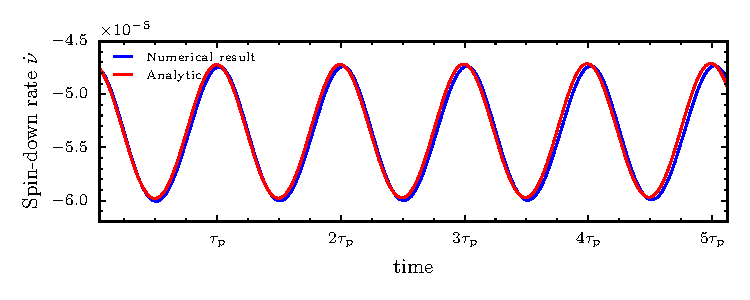
\includegraphics[]{SpindownRate_normal}
\caption{Spin-down rate for simulation parameters listed in Table~\ref{tab:
spin-down rate normal} compared against the corresponding analytic prediction
of Eqn.\eqref{eqn: spin-down rate}.}
\label{fig: spin-down rate normal}
\end{figure}

Figure~\ref{fig: spin-down rate normal} captures the essential features of the
spin-down rate of a precessing pulsar amplified by an EM torque. However, there
is a special case which produces the `double-peaked' spin-down rate which is
observed in PSR~B1828-11 \citep{Lyne2010} (see also Chapter~\ref{sec: testing
models}) and PSR~0919+06 \citep{Perera2015}.  This double-peak arises naturally
in the precession model when $\theta \ll 1$ and $\chi$ is close to $\pi/2$.
This can be seen directly from the $\mathcal{O}(\theta^{2})$ term in
Eqn.~\eqref{eqn: spin-down rate}: when $\chi \sim \pi/2$, we get a second
harmonic at $\tauP/2$. To illustrate this, we will repeat the simulation of
Figure~\ref{fig: spin-down rate normal}, but set $\chi=88^{\circ}$; the full
set of simulation parameters are listed in Table~\ref{tab: spin-down rate
orthog}.
The spin-down rate for this `almost orthogonal' dipole simulation is plotted
in the top panel of Figure~\ref{fig: spin-down rate orthog} and demonstrates the
distinctive double peak.

\begin{table}[htb]
\centering
\begin{tabular}{ccl}
\multicolumn{3}{c}{Simulation parameters} \\
\hline
$\omega_0$  &=& $10^{4}$ rad/s\\
$B_0$  &=& $10^{14}$ G \\
$\chi$  &=& 85$^{\circ}$ \\
$a_0$ &=& 10$^{\circ}$ \\
$\mathcal{A}_{\mathrm{EM}}$ &= & $75$
\end{tabular}

\caption{Simulation parameters for the spin-down rate plotted in Figure~\ref{fig:
spin-down rate orthog}.}
\label{tab: spin-down rate orthog}
\end{table}

\begin{figure}[htb]
\centering
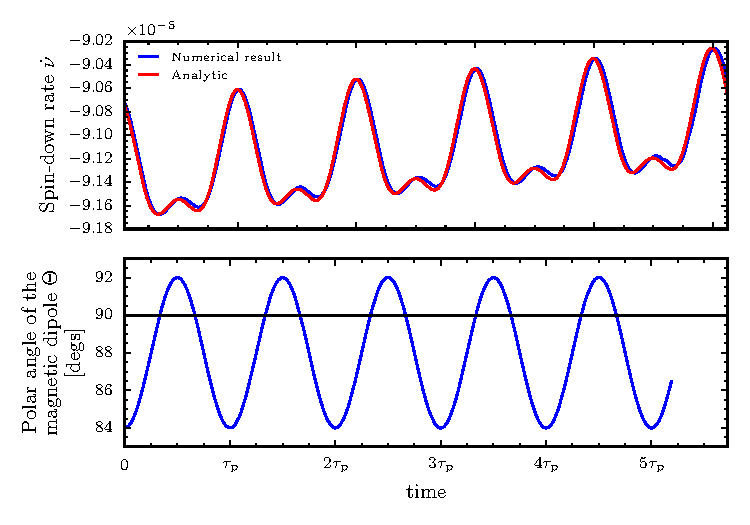
\includegraphics[]{SpindownRate_orthog}
\caption{Top panel: spin-down rate for simulation parameters listed in Table~\ref{tab:
spin-down rate orthog} compared against the corresponding analytic prediction
of Eqn.\eqref{eqn: spin-down rate}. This simulation differs from
Fig.~\ref{fig: spin-down rate normal} in that we chose $\chi$ such that the
magnetic dipole lies close to the rotation equator. Bottom panel: the variation
in the polar angle of the magnetic dipole, $\Theta$, for the simulation.}
\label{fig: spin-down rate orthog}
\end{figure}

We can understand this double-peaked feature by recalling that the dipole-cone
(introduced in Section~\ref{sec: understanding the motion of m}) is the
cone swept out by the magnetic dipole, $\m_a$, at the fast spin frequency; the
half-angle this cone makes with the angular momentum vector is $\Theta$ (see
Eqn.~\eqref{eqn: Theta 2}).  In the lower panel of Figure~\ref{fig: spin-down
rate orthog} we plot this polar angle for the same simulation. Notably the
occurrence of the double-peak in the spin-down rate coincides with times when
$\Theta > 90^{\circ}$. What we are seeing is the magnetic dipole entering the
lower hemisphere of the star. By considering the form of the
\citet{Deutsch1955} torque, we see that if the torque is maximal when the
dipole is perpendicular to the spin-vector. Since $\theta \ll 1$ and therefore
close to the angular momentum vector, we have a maximum in the torque and hence
spin-down rate when $\Theta \approx 90^{\circ}$. As $\Theta$ increases past
$90^{\circ}$ and the dipole enters the lower hemisphere, the absolute value
decreases again causing the distinctive double-peak in the spin-down rate.


\section{Observable features: the pulse profile}
\label{sec: observable features: shape}

So far we have considered physical observables which are calculable from the
timing properties of the star: the rate at which pulses occur. However, pulsar
astronomers also report on the shape of the pulsation by averaging over many
pulses to form an integrated pulse profile.  Long term variability in pulse
profiles is observed in pulsars. The correlated changes in shape for
PSR~B1828-11 allowed \citet{Stairs2000} to rule out a planetary precession
hypothesis. More examples of this variability can be found in \citet{Lyne2010}.

To quantify the changing shape of pulsations from PSR~B1828-11, astronomers
calculate the \emph{shape parameter} $S$. This is defined by first noting that
PSR~B1828-11 alternatives between two `modes', one narrow and one broad, then
defining $S$ as the fraction of the mean pulse shape attributed to the narrow
component (for more details see \citet{Stairs2003}). The effect of
precession on $S$ for a variety of beam geometries has been considered by
\citet{Akgun2006}.  However, this shape parameter is limiting as it requires
there to be two components.  A more general method was introduced by
\citet{Lyne2010} and defines the \emph{beam-width} as the width of the
pulsation at some fraction of the maximum observed intensity.

In the context of precession, the pulse profile is sensitive to both the
geometry of the beam itself and the angle made between the beam and the
observer.  Let us define an observer fixed in the inertial frame such that they
maintain a constant angle $\iota$ with the angular momentum of the star $J_a$.
For this observer, a pulse can be defined as the moment the dipole cuts through
the plane containing them and the angular momentum vector. At this moment, the
angle between them and the dipole will be determined by both $\iota \in [0, \pi]$ and
$\Theta \in [0, \pi]$. In particular, the angle between the observer and the beam
is given by
\begin{equation}
\Delta\Theta = \Theta - \iota.
\label{eqn: delta Theta}
\end{equation}
Since $\iota$ is fixed, variations in $\Delta\Theta$ come solely from
variations in the polar angle $\Theta$. We studied these variations in
Figure~\ref{fig: polar angle variations} and found that $\Theta$ has an
average value of the larger of $\theta$ or $\chi$, then oscillates about this
on the precession period with a magnitude given by the smaller value of
$\theta$ or $\chi$.

In this section, we aim to numerically simulate variations in the beam-width
due to precession. To do this, we first model variations in the pulse intensity
and then show how to model the determination of the beam-width. The process
described here, will be developed later in Chapter~\ref{sec: testing models} to
build a predictive analytic model for the beam-width of PSR~B1828-11.

\subsection{Variations in the pulse intensity}

The intensity of radiation received by an observer will depend on the
orientation of the magnetic dipole with respect to the observer and the beam
geometry. It may presumably be maximal when pointing directly at the observer
and fall off as the angle between the two grows. For each rotation of the star,
the intensity will peak when the beam cuts the plane containing the observer
and the angular momentum vector; at this instant the angle between the
observer and the beam is given by Eqn.~\eqref{eqn: delta Theta}. If the star is
precessing, then the periodic pulses of intensity due to the azimuthal rotation
of the star will be modulated by the slower variations in $\Theta$ seen in
Figure~\ref{fig: polar angle variations}.

To model this, we take an observer's azimuth and polar angle to be $(\PhiO,
\iota)$ and then assume the beam geometry follows a Gaussian profile with a
single conal emission.  This could later be adapted, for example to include
conal emission as modelled by \citet{Akgun2006}.  For such a model of the beam
geometry, the intensity of pulsations will vary with the angular separation of
the vector from the centre of the star to the observer and the magnetic dipole
vector. By considering the intersection of these vectors with the unit sphere,
the angular separation can be shown to be
\begin{equation}
\Delta d = \cos^{-1}\left(\cos(\Theta)\cos(\iota) +
                             \sin(\Theta)\sin(\iota)\cos(\Phi - \PhiO)\right)
\label{eqn: angular sep inv cos}
\end{equation}
Then, taking a Gaussian beam geometry, the intensity of the pulse will be given by
\begin{equation}
\mathcal{I}(\Theta, \Phi, \iota, \PhiO, \rho) =
\mathcal{I}_{0} \exp\left(-\frac{\Delta d^{2}(\Theta, \Phi, \iota, \PhiO)}{2\rho^{2}}\right)
\label{eqn: Gaussian beam intensity}
\end{equation}
where $\mathcal{I}_{0}$ is the maximum intensity and $\rho$ is a measure of the
width of the Gaussian intensity.

Given a value for $\mathcal{I}_0$ and $\rho$, we can use a numerical solution to the
governing ODEs to simulate this pulse intensity exactly. This is done in
Figure~\ref{fig: intensity variation} for a system where the variations in
$\Theta$ occur on a timescale not much longer than the pulse period. This
nonphysical simulation is intended to show the modulation of the individual
pulsations due to precession.
\begin{figure}[htb]
\centering
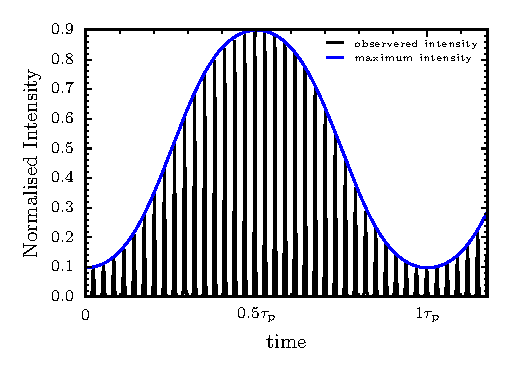
\includegraphics[width=.7\textwidth]{intensity_variation}
\caption{Amplitude variation using a 2D Gaussian emission.}
\label{fig: intensity variation}
\end{figure}
We can also predict the maximum pulse intensity at any given instant by setting
$\Phi=\PhiO$. Then simplifying, we find that
\begin{align}
\mathcal{I}_{\mathrm{max}}(\Theta, \Phi, \iota, \rho) =
\mathcal{I}_{0}\exp\left(\frac{-(\Theta-\iota)^{2}}{2\rho^{2}}\right),
\label{eqn: A max}
\end{align}
this is also shown in Figure~\ref{fig: intensity variation}.

\subsection{Variations in the beam-width}
\label{sec: numerical beam-width}
It is unlikely that the absolute variations in intensity seen in
Figure~\ref{fig: intensity variation} will ever be unambiguously visible in
nature. This is because in real observations the intensity will also be subject
to variations in the amount of scintillation from the interstellar medium.
Therefore, pulsar astronomers do not typically report on intensities
themselves, but characterise the pulsation by their beam-width. This is the
width of the pulse at some percentage $p$ of the observed maximum intensity.
Note that this is not the maximum intensity that the beam produces, $\mathcal{I}_0$, but
the maximum at that instant in time $\mathcal{I}_{\mathrm{max}}$, as given by
Eqn.~\eqref{eqn: A max}

To calculate the beam-width, we first note that in Eqn.~\eqref{eqn: Gaussian
beam intensity}, $\Theta$ varies on the slow precession timescale, while $\Phi$
varies on the rapid spin timescale: we are looking to measure the variations
with respect to the slow precession timescale.  The pulse width is measured by
the time spent above a percentage $p$ of the maximum pulse intensity, this can
be defined as an inequality
\begin{align}
\mathcal{I}(\Phi, \Theta, \iota, \PhiO, \rho) > \mathcal{I}_{\textrm{max}} \frac{p}{100}.
\end{align}
Substituting in Eqn.~\eqref{eqn: Gaussian beam intensity} and Eqn.~\eqref{eqn: A max}
then rearranging yields
\begin{equation}
\cos(\Phi - \PhiO) > \frac{
\cos\left(
\sqrt{-2\rho^{2}
\ln\left[\frac{p}{100}\frac{\mathcal{I}_\textrm{max}}{\mathcal{I}_0}\right]}\right) -
\cos(\Theta)\cos(\iota)} {\sin(\Theta)\sin(\iota)}
\label{eqn: 6737}
\end{equation}
where we note that $\mathcal{I}_\textrm{max}$ is not a constant, but will evolve with the
polar angle $\Theta$ as given by Eqn.~\eqref{eqn: Theta 2}.

Let's consider a single rotation with the magnetic dipole starting and ending in
the antipodal point to the observer's position. During this rotation, $\Phi -
\PhiO$ increases linearly between $-\pi$ and $\pi$, and so the left hand side of the
inequality is a simple cosine function as illustrated in Figure~\ref{fig:
CosineIllustration}.  Since we expect $\Theta$ to vary slowly compared to the
rotation period we can, over a single pulsation, think of $\Theta$ as a
constant; then the whole right hand side of Inequality~\eqref{eqn: 6737} is a
constant. In Figure~\ref{fig: CosineIllustration}, we illustrate this constant
along with the evolution of the left hand side. Then we also illustrate $\Delta\Phi$,
the fraction of the rotation period for which the cosine is less than the
constant, i.e. Inequality~\eqref{eqn: 6737} is satisfied.
\begin{figure}[ht]
\centering
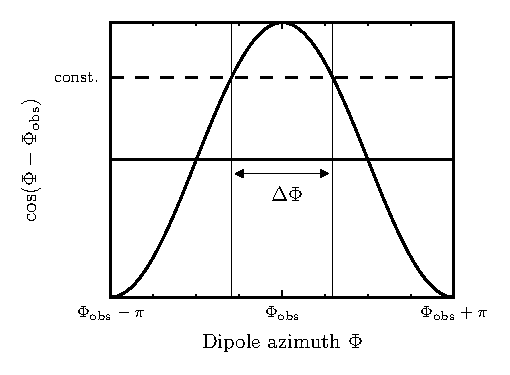
\includegraphics[width=.75\textwidth]{CosineIllustration.pdf}
\caption{Illustration of $\cos(\Phi-\PhiO)$ during a single rotation. The constant
         value represents the right hand side of this equation. The
         width $\Delta\Phi$ indicates the angular period during which
         Inequality~\eqref{eqn: 6737} is satisfied.}
\label{fig: CosineIllustration}
\end{figure}

The angular fraction at which the inequality \emph{is} satisfied is given by
$\Delta\Phi$. To convert this into the beam-width reported by pulsar
astronomers we multiply by the pulse period. So from $\Delta\Phi$, we can
calculate the beam-width as
\begin{align}
    W_{p} & = P \frac{\Delta\Phi}{2\pi}
\end{align}
where $P$ is the spin period.

The angular width $\Delta\Phi$ when the inequality is satisfied is given by
\begin{equation}
    \Delta\Phi = 2\cos^{-1}\left(
                \frac{
\cos\left(\sqrt{-2\rho^{2}\ln\left[\frac{p}{100}\frac{\mathcal{I}_{\mathrm{max}}}{\mathcal{I}_0}\right]}\right) - \cos(\Theta)\cos(\iota)}
                          {\sin(\Theta)\sin(\iota)}
                      \right),
\end{equation}
and so the beam-width is
\begin{align}
    W_{p} & = \frac{1}{\pi\dot{\Phi}}
               \cos^{-1}\left(
                   \frac{\cos\left(
\sqrt{-2\rho^{2}\ln\left[\frac{p}{100}\frac{A_{\mathrm{max}}}{A_0}\right]}
\right) - \cos(\Theta)\cos(\Theta)}
                          {\sin(\Theta)\sin(\iota)}
                  \right).
\end{align}
Finally, we can also simplify this results using Eqn.~\eqref{eqn: A max} to give
\begin{align}
    W_{p} & = \frac{1}{\pi\dot{\Phi}}
               \cos^{-1}\left(
                   \frac{\cos\left(
\sqrt{(\Theta-\iota)^2 - 2\rho^2 \ln\left(\frac{p}{100}\right)}
\right) - \cos(\Theta)\cos(\Theta)}
                          {\sin(\Theta)\sin(\iota)}
                  \right).
\label{eqn: Wp}
\end{align}


To demonstrate an example of the beam-width modulation, in Figure~\ref{fig: Pulse width
modulation} we plot $\Theta$ calculated from a numerical simulation with the
simulation parameter listed in Table~\ref{tab: pulse width modulation} and
$W_{10}$ as calculated from Eqn.~\eqref{eqn: Wp} with $\iota=82^{\circ}$ and
$\rho=0.3$.

\begin{table}[htb]
\centering
\begin{tabular}{ccl}
\multicolumn{3}{c}{Simulation parameters} \\
\hline
$\omega_0$  &=& 1.0 rad/s\\
$B_0$  &=& $0$ G \\
$\chi$  &=& 80.0$^{\circ}$ \\
$a_0$ &=& 6.0$^{\circ}$ \\
$\tilde{\theta}$ &= & 6.0$^{\circ}$ \\
$\mathcal{A}_{\mathrm{EM}}$ &= & $0$
\end{tabular}

\caption{Simulation parameters for the beam-width modulations plotted in
Figure~\ref{fig: Pulse width modulation}.}
\label{tab: pulse width modulation}
\end{table}

\begin{figure}[ht]
\centering
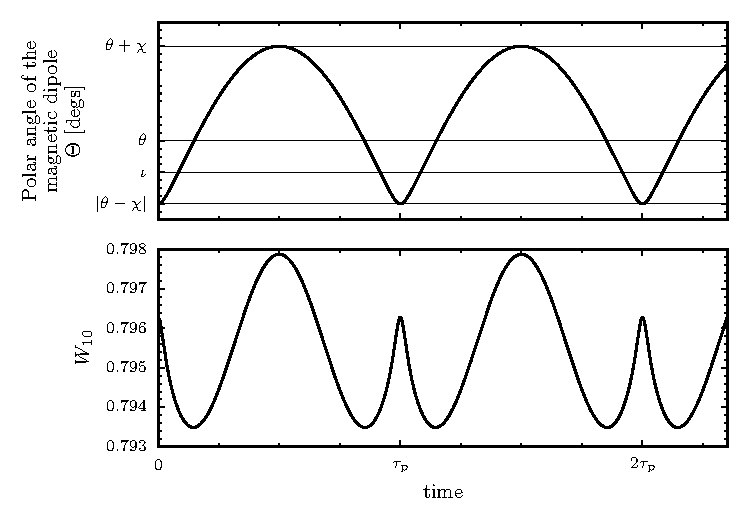
\includegraphics[]{Pulse_width_modulation.pdf}
\caption{Simulation results for the polar angle $\Theta$ and $W_{10}$, a
measure of the observed beam-width as calculated from Eqn.~\eqref{eqn: Wp}.
The simulation parameters for this are listed in Table~\ref{tab: pulse width modulation}
and we additionally set $\iota=82^{\circ}$ and $\rho=0.3$ when calculating~$W_{10}$.}
\label{fig: Pulse width modulation}
\end{figure}


This shows that there is periodic modulation of the beam-width, with an
interesting two-peak structure. This structure can be understood by realising
that the polar angle of the dipole $\Theta$ `passes over' the observer such
that for some of the precessional phase the observer views the beam from below,
and other from above. This leads to the two-peaked structure due to the
symmetry of the emission geometry. This is a special case which depends on
the choices of $\theta, \chi$, and $\iota$: more generally the beam-width has
a single period oscillatory behaviour.

This numerical approach to modelling the beam-width allows us to simulate the
effects of precession and probe how this manifests in our observations.  We
will use the methods discussed in this section later in Chapter~\ref{sec:
inertial frame} when developing and fitting a precession model for the
observed beam-width of PSR~B1828-11.


\section{Application: switching and precession}
\label{sec: application switching and precession}

Recently, some workers in the field \citep{Lyne2010, Perera2015} have suggested
that quasi-periodic structure observed in some pulsar timing residuals is a
result of magnetospheric torque-switching events as described in
Section~\ref{sec: two state switching}. In such models, the magnetospheric
torque, and hence spin-down rate periodically switches between two distinct
values and these changes correlate with changes in the beam-width.  These
models however are lacking a key feature: the clock which provides the
periodicity. It has been suggested \citep{Jones2012} that it may in fact be
precession which provides this clock. Ultimately, the numerical model developed
in this section could study this effect, for example by implementing a hybrid
model in which propensity for a magnetospheric switch to occur is related to
the angle $\Theta$. In this way, the observed switching would undergo
stochastic resonance as suggested by \citet{Cordes2013} and discussed in
Appendix~\ref{app: stochastic}.

In this section, we will present novel, but preliminary results on a simplified
hybrid magnetospheric switching - precession model. Ultimately we would like to
realise the ideas discussed above in a full numerical model. However, for now
we will simply consider the effect of a single magnetospheric torque switching
event. Our numerical code is able to model the full hybrid model, but we must
first understand the basic physics. In particular, we will simulate a star in
which at $t_{\mathrm{switch}} = \Tobs/2$ the EM torque suddenly decreases. This is
a qualitatively new idea which has not yet been discussed in the literature.

In the EM dipole spin-down model, the torque has two distinct components: the
regular spin-down component and the anomalous component. This latter term does
not contribute to the spin-down, but as discussed in Section~\ref{sec:
effective body frame} will modify the axis of precession. Magnetospheric
switching models are based on evidence that the spin-down rate is switching,
therefore the torque switching must occur in the spin-down component. However,
it is unclear if it will also occur in the anomalous component. To answer this,
one would need a detailed model of how the magnetosphere reconfigures during the
switching. We will not do this here, but instead investigate a simple
phenomenological switching event in which we modify Eqn.~\eqref{eqn: torque} as
follows

\newcommand{\Ss}{S_{\mathrm{S}}}
\newcommand{\Sa}{S_{\mathrm{A}}}

\begin{equation}
\mathbf{T} = (1 - \Ss H(t-t_{\mathrm{switch}})) \mathbf{T}_{\mathrm{S}}+
                 (1 - \Sa H(t-t_{\mathrm{switch}})) \mathbf{T}_{\mathrm{A}}
\label{eqn: single switch torque}
\end{equation}
where the subscripts label the spin-down and anomalous components, $S$ is the
strength of switching, and $H(t)$ is the Heaviside step function. In this model
we can control which components are switched by choosing $\Ss$ and $\Sa$
appropriately.

In our model the strength of the EM torque is parameterised
by $\epsA$, related to the surface magnetic field strength by
\begin{align}
    \epsA = \frac{R^{5}}{4I_{0} c^{2}} B_{0}^{2}.
\end{align}
Rearranging Eqn.~\eqref{eqn: surface magnetic field} we can then write the
spin-down rate as
\begin{align}
\begin{split}
    \dot{\omega}_{0} & = -\frac{B_{0}^{2}R^{6} \sin^{2}(\alpha) \omega_{0}^{3}}{6 I_{0} c^{3}} \\
    & = - \frac{2 R \epsA \sin^{2}(\alpha) \omega_{0}^{3}}{3 c},
\end{split}
\end{align}
where $\alpha$ is the angle between the spin-vector and magnetic dipole. Since
we expect these to be misaligned in order to observe pulsations, we can take
$\sin^{2}\alpha \approx 1$, then our spin-down rate is approximately
\begin{equation}
    \dot{\nu} = - \frac{R\omega_{0}^{3}}{3\pi c}\epsA.
    \label{eqn: spin-down of epsA}
\end{equation}

From this we can equate the switching in the spin-down rate $\Ss$ directly to
that measured from pulsar observations. That is, from Eqn.~\eqref{eqn: single switch torque}
we have that
\begin{equation}
    \epsA \rightarrow \epsA' = (1-\Ss)\epsA.
\label{eqn: epsA switch}
\end{equation}
Then the spin-down rate also changes as
\begin{equation}
    \dot{\nu} \rightarrow \dot{\nu}' = (1-\Ss)\dot{\nu}.
\label{eqn: nudot switch}
\end{equation}
during a switching event.

\subsubsection{Minimal precession initial state}
In the following section we will investigate the effects of a single switch, but
first we choose to define an initial `minimal precession' from which to begin
our simulations. This is done to mimic the state of real pulsars, which in
general are not found to be precessing. Moreover, it helps to discern the
effects of the switching from that of precession.

Precession will not occur when the spin-vector is aligned with the principal
axis of the effective moment of inertia tensor (defined in Sec.~\ref{sec:
effective body frame}). The angle between these is approximately the
effective wobble angle defined in Eqn.~\eqref{eqn: effective wobble angle}.
For minimal precession we should therefore set this wobble angle to
zero. In all simulations, we consider a biaxial body with the full torque given
by \eqref{eqn: single switch torque}. From our previous discussion on the
wobble angle we can minimise the precession initially by setting the initial polar angle
of the spin-vector in the rotating frame to lie along the effective body-frame
axis. In the presence of the anomalous torque this is done with
\begin{equation}
a_{0} = \beta(\epsI, \epsA, \chi),
\end{equation}
where $\beta$ is defined in Eqn.~\eqref{eqn: beta}.

In Figure~\ref{fig: no switching} we illustrate the phase residual of our
simulation in the absence of a switching event; the simulation parameters are
listed in Table~\ref{tab: switching props}. Note that the initial polar angle
is exactly the angle $\beta$ which can be calculated using Eqn.~\eqref{eqn:
beta}.

\begin{figure}[htb]
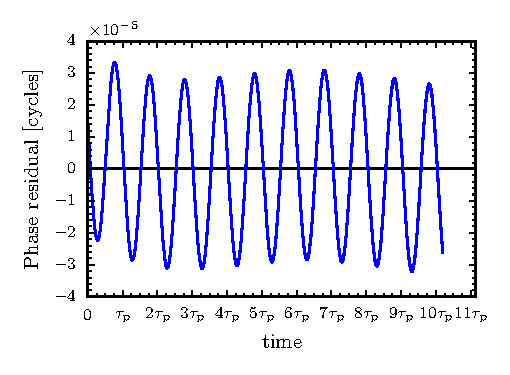
\includegraphics[width=0.5\textwidth]{NoSwitching.pdf}
\caption{The phase residual for a minimal precession simulation with no
         switching event; the simulation properties are listed in
         Table~\ref{tab: switching props}. In this case, we have fitted and
         removed a Taylor expansion up to and including $\ddot{\nu}$.
         Note that, due to inherent errors in the fitting process, the residual
         exhibits an apparent periodicity which matches its span (or some integer
         number of periods fits into the span, in this case 2). This was shown
         to be the case by varying the observation span and observing a
         corresponding shift in the period, as such it is a non-physical effect
         which can be ignored.
}
\label{fig: no switching}
\end{figure}

\begin{table}[htb]
\centering
\begin{tabular}{ccl}
\multicolumn{3}{c}{Simulation parameters} \\
\hline
$\omega_0$  &=& 100 rad/s\\
$B_0$  &=& $10^{15}$ G \\
$\chi$  &=& 50$^{\circ}$ \\
$a_0$ &=& -0.78$^{\circ}$ \\
$\mathcal{A}_{\mathrm{EM}}$ &= & $23$
\end{tabular}

\caption{Simulation properties used for Figure~\ref{fig: no switching},
Figure~\ref{fig: switching without anom}, and Figure~\ref{fig: switching with anom}.}
\label{tab: switching props}
\end{table}

Notably this minimal precession solution does show some precession with phase
residuals $\sim 10^{-5}$. This is because the spin-down torque produces a wobble
in the angular momentum vector and as a result the wobble angle is not truly
zero. For all the phase residuals calculated in this section, we will fit and
remove a Taylor expansion up to and including $\ddot{\nu}$.

We will now set up simulations of this `minimal precession` star, and then
manually switch the torque. We choose a star where the EM torque amplification is
important.  In the following sections, we will consider first switching in the
spin-down torque, and then also in the anomalous torque. For all simulations
considered here we will use the properties listed in Table~\ref{tab: switching
props}.

\subsection{Switching in the spin-down torque only}
We now consider manually switching the spin-down torque halfway though the
simulation, with no switch occurring in the anomalous component.
That is we set
\begin{align}
    t_{\mathrm{switch}} = \frac{\Tobs}{2}, &&& \Ss = 0.4, &&& \Sa = 0.0,
\label{eqn: SD only}
\end{align}
such that halfway though the simulation the spin-down torque is reduced by a
fraction $0.4$ while the anomalous torque remains unaffected.

In Figure~\ref{fig: switching without anom} we plot the phase residuals from
this simulation. In the top plot is the residual as calculated over the entire
observation period. We find a single periodic variation with a period of the
observation time $\Tobs$: due to sudden change in spin-down rate the Taylor
expansion fit is not finding a suitable fit. The precession features which
existed in the initial minimal precession are swamped by the larger variations
due to the switch. To study this simulation further, in the lower plot we plot
two residuals: the first is calculated in the region $[0, t_{\mathrm{switch}}]$
and the second in $[t_{\mathrm{switch}}, \Tobs]$. Because the switch does not
occur in either of these periods we can resolve the free precession during each
period and note that the precession modulation is in fact smaller after the
switch.
\begin{figure}[htb]
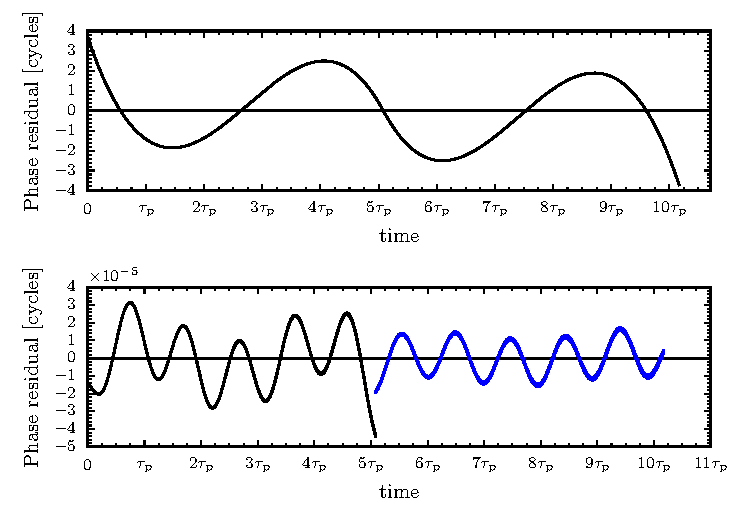
\includegraphics[]{SwitchingWithoutAnomTorque}
\caption{Phase residuals for a simulation with a single switch in the spin-down
torque with the parameters given in Eqn.~\eqref{eqn: SD only} and the
simulation properties listed in Table~\ref{tab: switching props}. In the top
plot we show the residual calculated using the whole observation time. The
bottom plot is the separate residuals calculated in the region before and after
the switch.}
\label{fig: switching without anom}
\end{figure}
This reduction in the size of modulations is because the precession is due to
the spin-down torque wobbling the angular moment vector and being amplified by
the EM torque. After the switch the spin-down torque, and hence $\Aem$, is
reduced by a factor $\Ss$ and therefore the size of the modulation is similarly
reduced.

\subsection{Switching in the spin-down and anomalous torque}
We now consider manually switching both the spin-down and anomalous torque
halfway though the simulation.  That is we set
\begin{align}
    t_{\mathrm{switch}} = \frac{\Tobs}{2}, &&& \Ss = \Sa = 0.01
\label{eqn: SD and A}
\end{align}

In a similar fashion to Figure~\ref{fig: switching without anom}, we first show
the total residual in the top plot of Figure~\ref{fig: switching with anom}, and
then the individual residuals in the lower plot. Again, the overall phase
residual exhibits periodic modulation with a period of the observation time $\Tobs$
resulting from the failing of the fitting algorithm to find an appropriate fit.
In contrast to the spin-down only switching, the amount of precession when
considered before and after the glitch now increases.

To understand this, recall that we begin with a minimal precession state, where
$\theta = \beta$ and the precession results from effect of the spin-down
torque.  After the switch, we have changed the size of the anomalous torque and
hence we have modified the effective body frame and the angle $\beta$. This
means that after the switch the star is no longer in a minimal
precession configuration.
This generates a significantly larger wobble angle producing a significant
increase in the phase residuals fitted in the post-switch period. The effect is
not observable when fitting to the entire simulation period since the switching
event remains dominant. In the next section we will calculate this new wobble
angle.
\begin{figure}[htb]
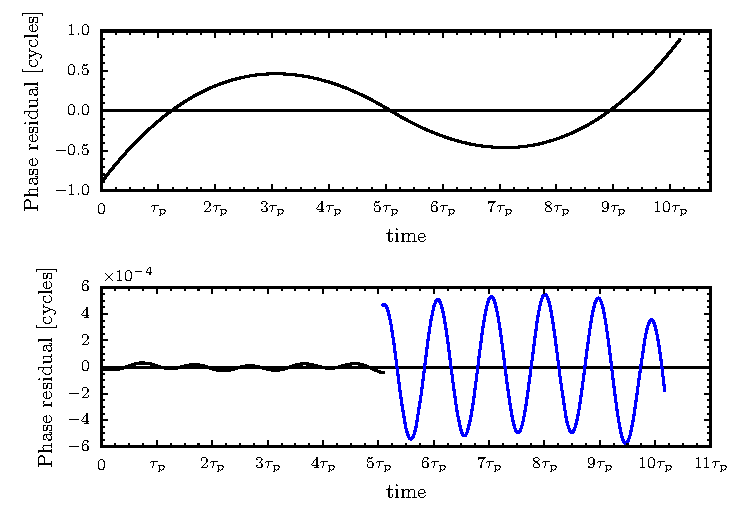
\includegraphics[]{SwitchingWithAnomTorque}
\caption{Phase residuals for a simulation with a single switch in the spin-down
and anomalous torque with the parameters given in Eqn.~\eqref{eqn: SD and A}
and the simulation parameters listed in Table~\ref{tab: switching props}. In
the top plot we show the residual calculated using the whole observation time.
The bottom plot is the separate residuals calculated in the region before
and after the switch.}
\label{fig: switching with anom}
\end{figure}

\subsubsection{Calculating the new wobble angle after a switch}
We now estimate the change in wobble angle after switching a fraction of the
anomalous torque. This will be useful in making testable predictions for
anomalous torque switching.

The two-state switching changes the value of $\epsA$ according to
Eqn.~\eqref{eqn: epsA switch}, which in turn redefined the effective rotating frame
as defined in Section~\ref{sec: effective body frame}. A non-precessing star at an
angle $\beta(\epsI, \epsA, \chi)$ will, after an anomalous torque switch by a fractional
amount $\Sa$, no longer be aligned with the rotating frame axis. This is
because the effective rotating frame will have shifted to $\beta' = \beta(\epsI,
\Sa\epsA, \chi)$. As a result, we should expect the previously
non-precessing star to begin precessing after a torque switching event.
The exact size of the new precession wobble angle will depend on the phase of
precession (if it was precessing) at the instant before the switching event.
The exact change in the wobble angle will depend on the precessional phase at
the time of the glitch, however, we can approximate it in a crude way by considering
\begin{equation}
    \Delta\beta(\epsI, \epsA, \chi, \Sa) \sim |\beta - \beta'|.
\label{eqn: d b}
\end{equation}
The expression for $\Delta \beta$ is not easily amenable to analytic
calculation, but can easily be explored graphically. In Figure~\ref{fig:
DeltaBetaPlot} we plot Eqn.~\eqref{eqn: d b} by calculating $\beta$ and
$\beta'$ values using Eqn.~\eqref{eqn: beta}; this is done for several choices
of $\Sa$ to show the typical variations. This illustrates that the new
precession angle after a switch can be as much as a few degrees although it
tends to zero in the limit $\epsI \gg \epsA$ and $\epsI \ll \epsA$.
\begin{figure}[htb]
    \centering
    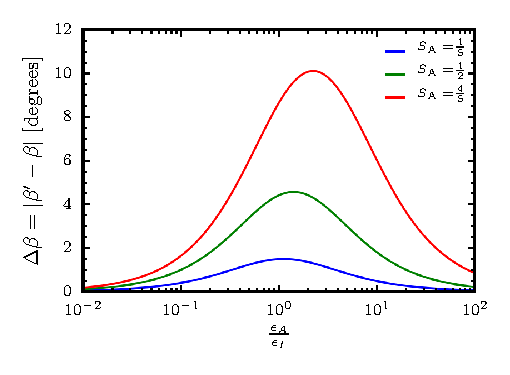
\includegraphics[]{DeltaBetaPlot}
    \caption{Illustrating the magnitude of the precession angle after switching
        due to the new rotation of the effective rotating frame. We plot the half-angle
        ($\Delta\beta$) of the precession cone as a function of the ratio
    $\epsA/\epsI$. Typically we expect real stars to have $\epsA < \epsI$.}
    \label{fig: DeltaBetaPlot}
\end{figure}

A simple application of this work is to apply our findings to PSR~B1828-11,
which was interpreted by \citet{Lyne2010} as undergoing switching with a fractional
change in the spin-down rate given by
\begin{align}
\frac{\Delta\dot{\nu}}{\dot{\nu}} = 0.007.
\end{align}
Manipulating Eqn.~\eqref{eqn: nudot switch}, we see that
\begin{align}
|\Ss| = \frac{\Delta\dot{\nu}}{\dot{\nu}}.
\end{align}
Using data from the ATNF catalogue \citep{ATNF}, PSR~B1828-11 has a frequency
$\nu = 2.47$~Hz, a spin-down rate $\dot{\nu}=-3.65\times10^{-13}$~Hz/s.
Rearranging Eqn.~\eqref{eqn: spin-down of epsA} we then have
\begin{align}
\epsA^{B1828-11} = \frac{c}{8\pi R\nu^{3}}\dot{\nu} \approx 3 \times 10^{-11}.
\end{align}

Now in this interpretation, $\epsI$ is unconstrained for PSR~B1828-11 since the
periodic modulations are assumed to be resulting from switching and not
precession. Nevertheless, we numerically maximise $\Delta\beta$ over $\epsI$ to
find
\begin{align}
\Delta\beta_{\textrm{max}}(\epsA=2.89\times10^{-11}, \epsI=2.87\times10^{-11})
= 0.05 \textrm{ degs}.
\end{align}
This is the maximum new wobble angle which must occur every time PSR~B1828-11 undergoes a
switching event, if the switch also occurs in the anomalous torque. This
therefore provides a method to probe how the switching mechanism works by
looking at timing residuals in the post-switch timing data to check for
any signs of precession.

\section{Conclusions}
\label{sec: conclusion inertial}

In this chapter, we have developed a method to simulate observable properties
of neutron stars by evolving the governing system of ODEs. These equations,
given in Eqn.~\eqref{eqn: 6ODE x} to Eqn.~\eqref{eqn: 6ODE psi}, contain both
the components of the spin-vector in the rotating frame and the Euler rotation
angles required to transform from the rotating frame to the inertial frame.
This step is important since it is in this reference frame that observers view
the effects of precession on the pulsar's observation features.

We developed an intuitive model for how the magnetic dipole, along which EM
radiation is emitted, moves in the inertial frame. Comparing with analytic
models where possible, we showed how to calculate from the motion of the
dipole the evolution of the star's timing properties (the phase, frequency, and
spin-down rate) and how to calculate features of the beam shape such as the
beam-width. In doing this, we derived the spin-down rate for a precessing pulsar
(see Section~\ref{sec: derivation of the spin-down rate}), which will be used in
Chapter~\ref{sec: testing models}, and verified it against numerical solutions.

Finally, we used the phase residuals to investigate the effect of a simple
torque switching model in which the components of the torque instantaneously
change.  This was done to model the magnetospheric switching which is proposed
by \citet{Lyne2010} as an explanation of the periodic modulation of
PSR~B1828-11. We present preliminary results showing the complicated
interactions which occur in single switching events; in the future we would
like to extend this to having the precession determine when the switching
occurs. Our numerical model is ideally suited to this task as it captures the
complicated feedback between precession and the changing torque.  Furthermore,
we would eventually like to link the switching to the precessional phase in
a probabilistic way as proposed by \citet{Jones2012}. In this way, precession
provides the clock to the switching. By virtue of being probabilistic, such a
system will display stochastic resonance as first described by
\citet{Cordes2013}.

\biblio

\end{document}
